\documentclass[8pt,aspectratio=169]{beamer}
\usetheme{Madrid}
\usepackage{graphicx,booktabs,adjustbox,multicol,amsmath,listings,xcolor}
\definecolor{mlblue}{RGB}{0,102,204}
\definecolor{mlpurple}{RGB}{51,51,178}
\definecolor{mllavender}{RGB}{173,173,224}
\definecolor{mllavender2}{RGB}{193,193,232}
\definecolor{mllavender3}{RGB}{204,204,235}
\definecolor{mllavender4}{RGB}{214,214,239}
\definecolor{mlorange}{RGB}{255,127,14}
\definecolor{mlgreen}{RGB}{44,160,44}
\definecolor{mlred}{RGB}{214,39,40}
\definecolor{mlgray}{RGB}{127,127,127}
\setbeamercolor{palette primary}{bg=mllavender3,fg=mlpurple}
\setbeamercolor{palette secondary}{bg=mllavender2,fg=mlpurple}
\setbeamercolor{palette tertiary}{bg=mllavender,fg=white}
\setbeamercolor{palette quaternary}{bg=mlpurple,fg=white}
\setbeamercolor{structure}{fg=mlpurple}
\setbeamercolor{title}{fg=mlpurple}
\setbeamercolor{frametitle}{fg=mlpurple,bg=mllavender3}
\setbeamercolor{block title}{bg=mllavender2,fg=mlpurple}
\setbeamercolor{block body}{bg=mllavender4,fg=black}
\setbeamertemplate{navigation symbols}{}
\setbeamertemplate{itemize items}[circle]
\setbeamersize{text margin left=5mm,text margin right=5mm}
\newcommand{\bottomnote}[1]{\vfill\vspace{-2mm}\textcolor{mllavender2}{\rule{\textwidth}{0.4pt}}\vspace{1mm}\footnotesize\textbf{#1}}
\lstdefinestyle{python}{language=Python,basicstyle=\ttfamily\tiny,keywordstyle=\color{mlblue}\bfseries,stringstyle=\color{mlgreen},commentstyle=\color{mlgray}\itshape,frame=single,backgroundcolor=\color{mllavender4},breaklines=true,tabsize=4,showstringspaces=false}
\lstset{style=python}
\usepackage{tikz,pgfplots}
\pgfplotsset{compat=1.18}
\usetikzlibrary{arrows.meta,positioning,shapes.geometric,calc,chains,decorations.pathmorphing,automata}
\title{Cryptography \& Security: A Quantitative Deep Dive}
\subtitle{Standalone Technical Lecture}
\author{Prof.~Dr.~Joerg Osterrieder}
\institute{University Lecture Series}
\date{\today}
\begin{document}

%--- FRAME 1: Title ---
\begin{frame}
\titlepage
\end{frame}

\section{Introduction and Motivation}

%--- FRAME 2: History of Cryptography Timeline ---
\begin{frame}{History of Cryptography Timeline}
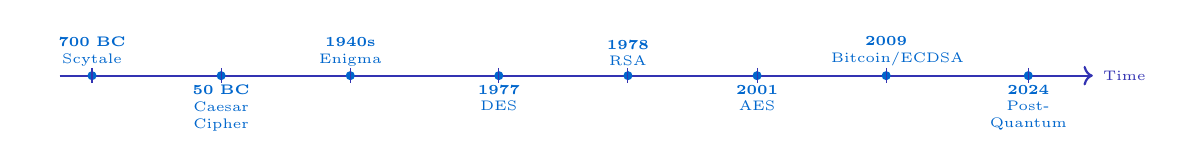
\begin{tikzpicture}[scale=0.82]
  \draw[->,thick,mlpurple] (0,0) -- (16,0) node[right]{\tiny Time};
  \foreach \x/\yr/\pos/\lbl in {
    0.5/700 BC/above/Scytale,
    2.5/50 BC/below/Caesar Cipher,
    4.5/1940s/above/Enigma,
    6.8/1977/below/DES,
    8.8/1978/above/RSA,
    10.8/2001/below/AES,
    12.8/2009/above/{Bitcoin/ECDSA},
    15.0/2024/below/Post-Quantum}{
    \fill[mlblue] (\x,0) circle(2pt);
    \draw[mlpurple] (\x,0.12)--(\x,-0.12);
    \node[\pos,font=\tiny,mlblue,align=center,text width=1.4cm] at (\x,0) {\textbf{\yr}\\\lbl};
  }
\end{tikzpicture}
\vspace{2mm}
\begin{columns}
\column{0.48\textwidth}
\begin{block}{Classical Era}
\begin{itemize}\small
  \item \textbf{700 BC}: Spartan scytale -- first transposition cipher
  \item \textbf{50 BC}: Caesar cipher -- substitution with shift key
  \item \textbf{1940s}: Enigma broken by Turing et al.
  \item \textbf{1977}: DES standardized (56-bit key)
\end{itemize}
\end{block}
\column{0.48\textwidth}
\begin{block}{Modern Era}
\begin{itemize}\small
  \item \textbf{1978}: RSA -- first practical public-key system
  \item \textbf{2001}: AES replaces DES (128/192/256-bit keys)
  \item \textbf{2009}: Bitcoin uses ECDSA on secp256k1
  \item \textbf{2024}: NIST post-quantum standards finalized
\end{itemize}
\end{block}
\end{columns}
\bottomnote{3000 years of cryptography: from physical devices to mathematical proofs of security}
\end{frame}

%--- FRAME 3: Kerckhoffs's Principle ---
\begin{frame}{Kerckhoffs's Principle}
\begin{columns}
\column{0.48\textwidth}
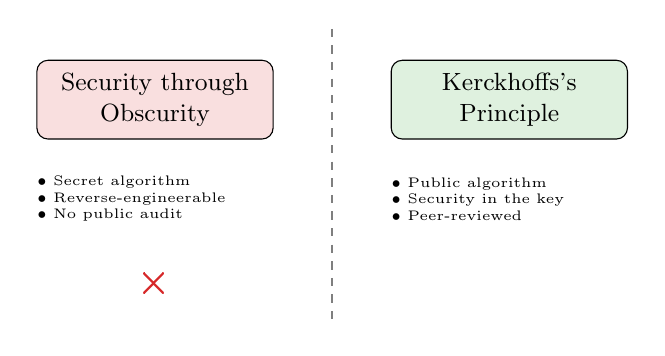
\begin{tikzpicture}[scale=0.9,
  box/.style={draw,rounded corners,minimum width=3cm,minimum height=1cm,font=\small,align=center}]
  % Security through Obscurity path
  \node[box,fill=mlred!15] (obs) at (0,3) {Security through\\Obscurity};
  \node[font=\tiny,align=left,text width=3cm] at (0,1.6) {
    $\bullet$ Secret algorithm\\
    $\bullet$ Reverse-engineerable\\
    $\bullet$ No public audit
  };
  \node[font=\Large,mlred] at (0,0.4) {\textbf{\texttimes}};
  % Kerckhoffs path
  \node[box,fill=mlgreen!15] (ker) at (5,3) {Kerckhoffs's\\Principle};
  \node[font=\tiny,align=left,text width=3cm] at (5,1.6) {
    $\bullet$ Public algorithm\\
    $\bullet$ Security in the key\\
    $\bullet$ Peer-reviewed
  };
  \node[font=\Large,mlgreen] at (5,0.4) {\checkmark};
  % Dividing line
  \draw[dashed,mlgray,thick] (2.5,4) -- (2.5,-0.2);
\end{tikzpicture}
\column{0.48\textwidth}
\begin{block}{Formal Statement}
\small A cryptosystem should be secure even if everything about the system, except the \textbf{key}, is public knowledge.
\end{block}
\vspace{2mm}
\begin{block}{Implications for Blockchain}
\begin{itemize}\small
  \item Bitcoin Core is \textbf{open source} -- anyone can audit
  \item Security rests on \textbf{private key secrecy}, not code secrecy
  \item Thousands of researchers verify cryptographic assumptions
  \item Obscure protocols often hide vulnerabilities
\end{itemize}
\end{block}
\begin{alertblock}{Key Insight}
\small Open algorithms with secret keys $\gg$ secret algorithms with no review.
\end{alertblock}
\end{columns}
\bottomnote{Auguste Kerckhoffs (1883): ``The system must not require secrecy and can be stolen by the enemy without causing trouble.''}
\end{frame}

%--- FRAME 4: Threat Model & Attack Taxonomy ---
\begin{frame}{Threat Model \& Attack Taxonomy}
\begin{columns}
\column{0.52\textwidth}
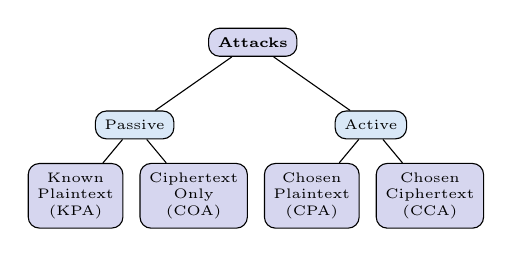
\begin{tikzpicture}[
  scale=0.75,
  level 1/.style={sibling distance=4cm,level distance=1.4cm},
  level 2/.style={sibling distance=2cm,level distance=1.2cm},
  every node/.style={font=\tiny,align=center},
  root/.style={draw,rounded corners,fill=mlpurple!20,font=\tiny\bfseries},
  cat/.style={draw,rounded corners,fill=mlblue!15},
  leaf/.style={draw,rounded corners,fill=mllavender4}
]
\node[root] {Attacks}
  child {node[cat] {Passive}
    child {node[leaf] {Known\\Plaintext\\(KPA)}}
    child {node[leaf] {Ciphertext\\Only\\(COA)}}
  }
  child {node[cat] {Active}
    child {node[leaf] {Chosen\\Plaintext\\(CPA)}}
    child {node[leaf] {Chosen\\Ciphertext\\(CCA)}}
  };
\end{tikzpicture}
\column{0.44\textwidth}
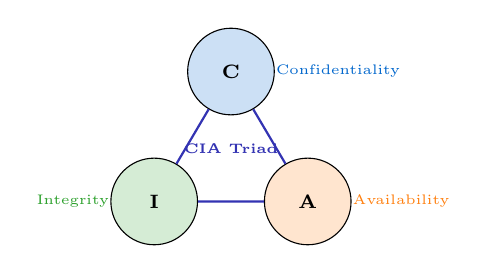
\begin{tikzpicture}[scale=0.75]
  % CIA triad
  \node[draw,circle,fill=mlblue!20,minimum size=1.1cm,font=\scriptsize\bfseries] (C) at (0,2.2) {C};
  \node[draw,circle,fill=mlgreen!20,minimum size=1.1cm,font=\scriptsize\bfseries] (I) at (-1.3,0) {I};
  \node[draw,circle,fill=mlorange!20,minimum size=1.1cm,font=\scriptsize\bfseries] (A) at (1.3,0) {A};
  \draw[thick,mlpurple] (C)--(I)--(A)--(C);
  \node[font=\tiny,mlblue,right] at (0.6,2.2) {Confidentiality};
  \node[font=\tiny,mlgreen,left] at (-1.9,0) {Integrity};
  \node[font=\tiny,mlorange,right] at (1.9,0) {Availability};
  \node[font=\tiny\bfseries,mlpurple] at (0,0.9) {CIA Triad};
\end{tikzpicture}
\end{columns}
\vspace{2mm}
\begin{columns}
\column{0.48\textwidth}
\begin{block}{Attack Hierarchy (Strength)}
\begin{itemize}\small
  \item COA $\subset$ KPA $\subset$ CPA $\subset$ CCA
  \item Scheme secure under CCA $\Rightarrow$ secure under all weaker models
  \item Modern goal: \textbf{IND-CCA2} (indistinguishability under adaptive CCA)
\end{itemize}
\end{block}
\column{0.48\textwidth}
\begin{block}{CIA in Blockchain Context}
\begin{itemize}\small
  \item \textbf{C}: Private keys, transaction privacy (zk-proofs)
  \item \textbf{I}: Hash chains, Merkle proofs, digital signatures
  \item \textbf{A}: P2P network, no single point of failure
\end{itemize}
\end{block}
\end{columns}
\bottomnote{A well-defined threat model is prerequisite for any formal security analysis}
\end{frame}

%--- FRAME 5: Course Roadmap ---
\begin{frame}{Course Roadmap}
\begin{columns}
\column{0.5\textwidth}
\begin{block}{8 Sections}
\begin{enumerate}\small
  \item \textcolor{mlpurple}{\textbf{Introduction \& Motivation}} \checkmark
  \item \textbf{Hash Functions Deep Dive} -- SHA-256, SHA-3, birthday bound
  \item \textbf{Symmetric Cryptography} -- AES, modes, DH key exchange
  \item \textbf{Asymmetric Cryptography} -- RSA, ECC, ECDSA
  \item \textbf{Digital Signatures} -- Schnorr, multisig, BLS
  \item \textbf{Key Management} -- HD wallets, BIP-32/39/44
  \item \textbf{Zero-Knowledge Proofs} -- zk-SNARKs, zk-STARKs
  \item \textbf{Post-Quantum Crypto} -- lattices, hash-based sigs
\end{enumerate}
\end{block}
\column{0.46\textwidth}
\begin{block}{Learning Objectives}
\begin{itemize}\small
  \item Master hash function internals and security proofs
  \item Understand elliptic curve mathematics for ECDSA
  \item Analyze key derivation and wallet security
  \item Evaluate zero-knowledge proof systems
  \item Assess post-quantum migration strategies
\end{itemize}
\end{block}
\vspace{2mm}
\begin{alertblock}{Central Question}
\small How do cryptographic primitives enable trustless digital ownership and verifiable computation?
\end{alertblock}
\end{columns}
\bottomnote{Prerequisites: modular arithmetic, basic group theory, probability}
\end{frame}

\section{Hash Functions Deep Dive}

%--- FRAME 6: Hash Function Formal Properties ---
\begin{frame}{Hash Function Formal Properties}
\begin{block}{Definition}
\small A cryptographic hash function $H:\{0,1\}^{*} \to \{0,1\}^{n}$ maps arbitrary-length input to a fixed $n$-bit digest.
\end{block}
\vspace{1mm}
\begin{columns}
\column{0.48\textwidth}
\begin{block}{Three Security Properties}
\begin{enumerate}\small
  \item \textbf{Preimage Resistance:}
    Given $y$, it is computationally infeasible to find $x$ s.t.\ $H(x)=y$.\\
    Complexity: $\mathcal{O}(2^{n})$
  \item \textbf{Second Preimage Resistance:}
    Given $x_1$, infeasible to find $x_2 \neq x_1$ s.t.\ $H(x_1)=H(x_2)$.\\
    Complexity: $\mathcal{O}(2^{n})$
  \item \textbf{Collision Resistance:}
    Infeasible to find \emph{any} $x_1 \neq x_2$ with $H(x_1)=H(x_2)$.\\
    Complexity: $\mathcal{O}(2^{n/2})$ (birthday bound)
\end{enumerate}
\end{block}
\column{0.48\textwidth}
\begin{block}{Property Hierarchy}
\begin{center}
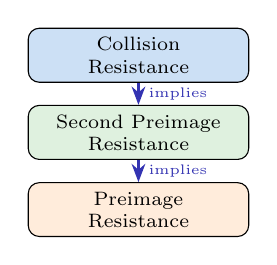
\begin{tikzpicture}[scale=0.7,
  box/.style={draw,rounded corners,fill=mllavender4,font=\scriptsize,minimum width=2.8cm,align=center}]
  \node[box,fill=mlblue!20] (cr) at (0,2.8) {Collision\\Resistance};
  \node[box,fill=mlgreen!15] (spr) at (0,1.4) {Second Preimage\\Resistance};
  \node[box,fill=mlorange!15] (pr) at (0,0) {Preimage\\Resistance};
  \draw[-{Stealth},thick,mlpurple] (cr) -- (spr) node[midway,right,font=\tiny]{implies};
  \draw[-{Stealth},thick,mlpurple] (spr) -- (pr) node[midway,right,font=\tiny]{implies};
\end{tikzpicture}
\end{center}
\end{block}
\vspace{1mm}
\begin{alertblock}{Note}
\small Collision resistance is the \emph{strongest} property. A collision-resistant hash is automatically second-preimage and preimage resistant.
\end{alertblock}
\end{columns}
\bottomnote{SHA-256 ($n=256$): preimage attack requires $\sim 2^{256}$ operations -- far beyond any computational budget}
\end{frame}

%--- FRAME 7: Merkle-Damgard Construction ---
\begin{frame}{Merkle--Damg\r{a}rd Construction}
\begin{center}
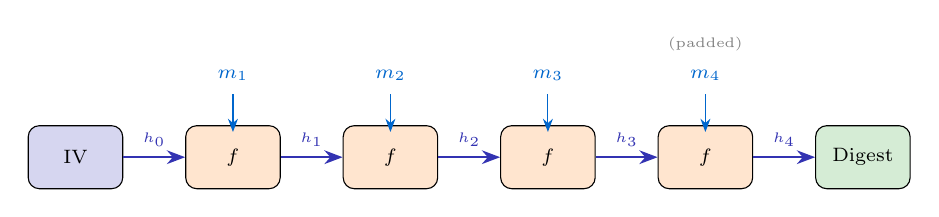
\begin{tikzpicture}[scale=0.8,
  block/.style={draw,rounded corners,fill=mlblue!15,minimum width=1.2cm,minimum height=0.8cm,font=\scriptsize},
  fblock/.style={draw,rounded corners,fill=mlorange!20,minimum width=1.2cm,minimum height=0.8cm,font=\scriptsize\bfseries}]
  % IV
  \node[block,fill=mlpurple!20] (iv) at (0,0) {IV};
  % Compression functions
  \node[fblock] (f1) at (2.5,0) {$f$};
  \node[fblock] (f2) at (5.0,0) {$f$};
  \node[fblock] (f3) at (7.5,0) {$f$};
  \node[fblock] (f4) at (10.0,0) {$f$};
  % Digest
  \node[block,fill=mlgreen!20] (digest) at (12.5,0) {Digest};
  % Arrows
  \draw[-{Stealth},thick,mlpurple] (iv) -- (f1) node[midway,above,font=\tiny]{$h_0$};
  \draw[-{Stealth},thick,mlpurple] (f1) -- (f2) node[midway,above,font=\tiny]{$h_1$};
  \draw[-{Stealth},thick,mlpurple] (f2) -- (f3) node[midway,above,font=\tiny]{$h_2$};
  \draw[-{Stealth},thick,mlpurple] (f3) -- (f4) node[midway,above,font=\tiny]{$h_3$};
  \draw[-{Stealth},thick,mlpurple] (f4) -- (digest) node[midway,above,font=\tiny]{$h_4$};
  % Message blocks (inputs from top)
  \foreach \i/\x in {1/2.5,2/5.0,3/7.5,4/10.0}{
    \node[font=\scriptsize,mlblue] at (\x,1.3) {$m_{\i}$};
    \draw[-{Stealth},mlblue] (\x,1.0) -- (\x,0.4);
  }
  % Padding note
  \node[font=\tiny,mlgray,align=center] at (10.0,1.8) {(padded)};
\end{tikzpicture}
\end{center}
\vspace{1mm}
\begin{columns}
\column{0.48\textwidth}
\begin{block}{Algorithm}
\begin{enumerate}\small
  \item Pad message $M$ to multiple of block size (512 bits for SHA-256)
  \item Split into blocks $m_1, m_2, \ldots, m_L$
  \item Initialize $h_0 = \text{IV}$ (fixed constants)
  \item Iterate: $h_i = f(h_{i-1}, m_i)$ for $i = 1,\ldots,L$
  \item Output: $H(M) = h_L$
\end{enumerate}
\end{block}
\column{0.48\textwidth}
\begin{block}{Security Reduction}
\small If $f$ is a collision-resistant compression function, then the full Merkle--Damg\r{a}rd hash $H$ is also collision-resistant.
\end{block}
\vspace{1mm}
\begin{alertblock}{Length Extension Weakness}
\small Given $H(M)$ and $|M|$, one can compute $H(M \| \text{pad} \| M')$ \textbf{without knowing} $M$. This is why HMAC or SHA-3 is preferred for MACs.
\end{alertblock}
\end{columns}
\bottomnote{SHA-256, SHA-512, MD5, and RIPEMD-160 all use Merkle--Damg\r{a}rd; SHA-3 uses the sponge construction instead}
\end{frame}

%--- FRAME 8: SHA-256 Internals ---
\begin{frame}{SHA-256 Internals: Compression Round}
\begin{center}
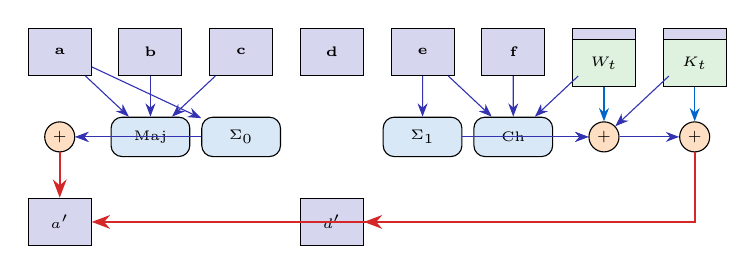
\begin{tikzpicture}[scale=0.72,
  reg/.style={draw,fill=mllavender4,minimum width=0.8cm,minimum height=0.6cm,font=\tiny\bfseries},
  op/.style={draw,circle,fill=mlorange!25,inner sep=1.5pt,font=\tiny\bfseries},
  func/.style={draw,rounded corners,fill=mlblue!15,font=\tiny,minimum width=1.0cm,minimum height=0.5cm}]
  % State variables
  \foreach \v/\i in {a/0,b/1,c/2,d/3,e/4,f/5,g/6,h/7}{
    \node[reg] (\v) at (\i*1.6,3) {\v};
  }
  % Functions
  \node[func] (ch) at (8.0,1.5) {Ch};
  \node[func] (sig1) at (6.4,1.5) {$\Sigma_1$};
  \node[func] (maj) at (1.6,1.5) {Maj};
  \node[func] (sig0) at (3.2,1.5) {$\Sigma_0$};
  % Addition nodes
  \node[op] (add1) at (9.6,1.5) {$+$};
  \node[op] (add2) at (11.2,1.5) {$+$};
  \node[op] (add3) at (0,1.5) {$+$};
  % Inputs
  \node[reg,fill=mlgreen!15] (kt) at (11.2,2.8) {$K_t$};
  \node[reg,fill=mlgreen!15] (wt) at (9.6,2.8) {$W_t$};
  % Connections
  \draw[-{Stealth},mlpurple] (e) -- (sig1);
  \draw[-{Stealth},mlpurple] (e) -- (ch);
  \draw[-{Stealth},mlpurple] (f) -- (ch);
  \draw[-{Stealth},mlpurple] (g) -- (ch);
  \draw[-{Stealth},mlpurple] (h) -- (add1);
  \draw[-{Stealth},mlpurple] (ch) -- (add1);
  \draw[-{Stealth},mlpurple] (sig1) -- (add1);
  \draw[-{Stealth},mlblue] (wt) -- (add1);
  \draw[-{Stealth},mlblue] (kt) -- (add2);
  \draw[-{Stealth},mlpurple] (add1) -- (add2);
  \draw[-{Stealth},mlpurple] (a) -- (sig0);
  \draw[-{Stealth},mlpurple] (a) -- (maj);
  \draw[-{Stealth},mlpurple] (b) -- (maj);
  \draw[-{Stealth},mlpurple] (c) -- (maj);
  \draw[-{Stealth},mlpurple] (sig0) -- (add3);
  \draw[-{Stealth},mlpurple] (maj) -- (add3);
  % New state arrows
  \node[reg] (d2) at (4.8,0) {$d'$};
  \node[reg] (a2) at (0,0) {$a'$};
  \draw[-{Stealth},thick,mlred] (add2) |- (d2);
  \draw[-{Stealth},thick,mlred] (add3) -- (a2);
  \draw[-{Stealth},thick,mlred] (add2) |- (a2);
\end{tikzpicture}
\end{center}
\vspace{1mm}
\begin{columns}
\column{0.48\textwidth}
\begin{block}{Round Operations (64 rounds)}
\begin{itemize}\scriptsize
  \item $\text{Ch}(e,f,g) = (e \wedge f) \oplus (\neg e \wedge g)$
  \item $\text{Maj}(a,b,c) = (a \wedge b) \oplus (a \wedge c) \oplus (b \wedge c)$
  \item $\Sigma_0(a) = \text{ROTR}^2(a) \oplus \text{ROTR}^{13}(a) \oplus \text{ROTR}^{22}(a)$
  \item $\Sigma_1(e) = \text{ROTR}^6(e) \oplus \text{ROTR}^{11}(e) \oplus \text{ROTR}^{25}(e)$
\end{itemize}
\end{block}
\column{0.48\textwidth}
\begin{block}{Parameters}
\begin{itemize}\scriptsize
  \item Block size: 512 bits (16 words of 32 bits)
  \item Digest: 256 bits (8 words)
  \item Rounds: 64 per block
  \item $K_t$: 64 round constants (fractional parts of cube roots of first 64 primes)
  \item $W_t$: message schedule (expanded from 16 to 64 words)
\end{itemize}
\end{block}
\end{columns}
\bottomnote{SHA-256 processes each 512-bit block through 64 rounds of mixing, shifting, and modular addition}
\end{frame}

%--- FRAME 9: Sponge Construction (Keccak/SHA-3) ---
\begin{frame}{Sponge Construction (Keccak / SHA-3)}
\begin{center}
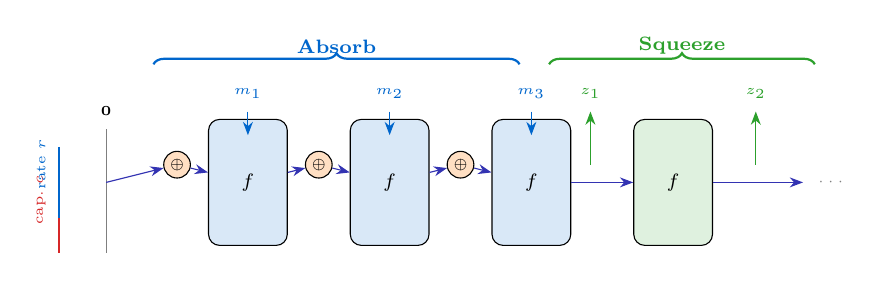
\begin{tikzpicture}[scale=0.75,
  block/.style={draw,rounded corners,fill=mlblue!15,minimum width=1.0cm,minimum height=1.6cm,font=\scriptsize\bfseries},
  state/.style={draw,minimum width=0.4cm,font=\tiny}]
  % Rate and capacity labels
  \draw[mlblue,thick] (-0.8,0.6) -- (-0.8,-0.6);
  \node[font=\tiny,mlblue,rotate=90] at (-1.1,0.3) {rate $r$};
  \node[font=\tiny,mlred,rotate=90] at (-1.1,-0.3) {cap.\ $c$};
  \draw[mlred,thick] (-0.8,-0.6) -- (-0.8,-1.2);
  % Initial state
  \node[font=\tiny] at (0,1.2) {\textbf{0}};
  \draw[mlgray] (0,0.9) -- (0,-1.2);
  % Absorb phase
  \foreach \i in {1,2,3}{
    \pgfmathsetmacro{\x}{\i*2.4}
    \node[block] (f\i) at (\x,0) {$f$};
    \node[font=\tiny,mlblue] at (\x,1.5) {$m_{\i}$};
    \draw[-{Stealth},mlblue] (\x,1.2) -- (\x,0.8);
    % XOR node
    \node[draw,circle,fill=mlorange!25,inner sep=1pt,font=\tiny] (xor\i) at (\x-1.2,0.3) {$\oplus$};
    \draw[-{Stealth},mlpurple] (xor\i) -- (f\i);
  }
  % Connect absorb chain
  \draw[-{Stealth},mlpurple] (0,0) -- (xor1);
  \draw[-{Stealth},mlpurple] (f1) -- (xor2);
  \draw[-{Stealth},mlpurple] (f2) -- (xor3);
  % Squeeze phase
  \node[block,fill=mlgreen!15] (f4) at (9.6,0) {$f$};
  \draw[-{Stealth},mlpurple] (f3) -- (f4);
  \node[font=\tiny,mlgreen] at (8.2,1.5) {$z_1$};
  \draw[-{Stealth},mlgreen] (8.2,0.3) -- (8.2,1.2);
  \node[font=\tiny,mlgreen] at (11.0,1.5) {$z_2$};
  \draw[-{Stealth},mlgreen] (11.0,0.3) -- (11.0,1.2);
  \draw[-{Stealth},mlpurple] (f4) -- (11.8,0);
  \node[font=\tiny,mlgray] at (12.3,0) {$\cdots$};
  % Phase labels
  \draw[decorate,decoration={brace,amplitude=4pt},mlblue,thick] (0.8,2.0) -- (7.0,2.0) node[midway,above,font=\scriptsize\bfseries]{Absorb};
  \draw[decorate,decoration={brace,amplitude=4pt},mlgreen,thick] (7.5,2.0) -- (12.0,2.0) node[midway,above,font=\scriptsize\bfseries]{Squeeze};
\end{tikzpicture}
\end{center}
\vspace{1mm}
\begin{columns}
\column{0.48\textwidth}
\begin{block}{Sponge Parameters}
\begin{itemize}\small
  \item State width: $b = r + c = 1600$ bits
  \item Rate $r$: bits absorbed/squeezed per call to $f$
  \item Capacity $c$: security parameter ($c = 2 \times$ security level)
  \item SHA3-256: $r=1088$, $c=512$, security $= 128$ bits
\end{itemize}
\end{block}
\column{0.48\textwidth}
\begin{block}{Advantages over Merkle--Damg\r{a}rd}
\begin{itemize}\small
  \item \textbf{No length extension attacks} by design
  \item Variable output length (SHAKE128, SHAKE256)
  \item Simpler security proof: random permutation model
  \item Algebraically distinct from SHA-2 (defense in depth)
\end{itemize}
\end{block}
\end{columns}
\bottomnote{Keccak won the NIST SHA-3 competition (2012) among 64 submissions; standardized as FIPS 202}
\end{frame}

%--- FRAME 10: Birthday Bound & Collision Probability ---
\begin{frame}{Birthday Bound \& Collision Probability}
\begin{columns}
\column{0.52\textwidth}
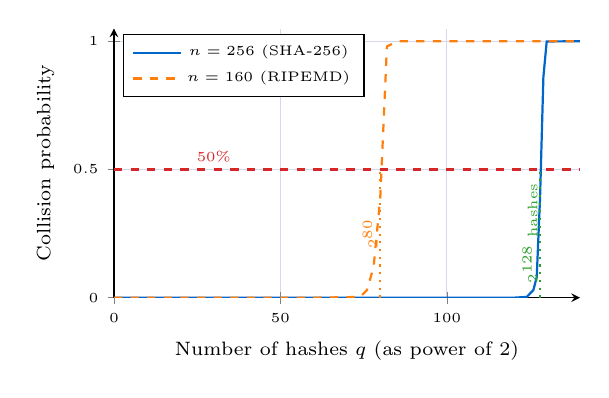
\begin{tikzpicture}
\begin{axis}[
  width=7.5cm, height=5.0cm,
  xlabel={\scriptsize Number of hashes $q$ (as power of 2)},
  ylabel={\scriptsize Collision probability},
  xmin=0, xmax=140,
  ymin=0, ymax=1.05,
  grid=major,
  grid style={mllavender4},
  axis lines=left,
  xlabel style={font=\scriptsize},
  ylabel style={font=\scriptsize},
  tick label style={font=\tiny},
  legend style={font=\tiny,at={(0.02,0.98)},anchor=north west}
]
% Collision probability curve (pre-computed to avoid pgfplots overflow)
% SHA-256: P ~ 1 - exp(-2^(2x-257))
\addplot[mlblue,thick] coordinates {
  (0,0)(60,0)(100,0)(120,0)(124,0.003)(126,0.03)(127,0.08)
  (128,0.39)(129,0.86)(130,0.9997)(135,1)(140,1)
};
\addlegendentry{$n=256$ (SHA-256)}
% RIPEMD-160: P ~ 1 - exp(-2^(2x-161))
\addplot[mlorange,thick,dashed] coordinates {
  (0,0)(40,0)(60,0)(74,0.003)(76,0.03)(78,0.12)
  (80,0.39)(82,0.98)(85,1)(100,1)(140,1)
};
\addlegendentry{$n=160$ (RIPEMD)}
% Mark the 50% line
\draw[mlred,dashed,thick] (axis cs:0,0.5) -- (axis cs:140,0.5);
\node[font=\tiny,mlred] at (axis cs:30,0.55) {50\%};
% Mark 2^128 for SHA-256
\draw[mlgreen,thick,dotted] (axis cs:128,0) -- (axis cs:128,0.5);
\node[font=\tiny,mlgreen,rotate=90] at (axis cs:125,0.25) {$2^{128}$ hashes};
% Mark 2^80 for RIPEMD-160
\draw[mlorange,thick,dotted] (axis cs:80,0) -- (axis cs:80,0.5);
\node[font=\tiny,mlorange,rotate=90] at (axis cs:77,0.25) {$2^{80}$};
\end{axis}
\end{tikzpicture}
\column{0.44\textwidth}
\begin{block}{Birthday Paradox}
\small For $N = 2^n$ possible outputs and $q$ queries:
\[P(\text{collision}) \approx 1 - e^{-q^2/(2N)}\]
At $q \approx \sqrt{N} = 2^{n/2}$, probability $\approx 50\%$.
\end{block}
\vspace{1mm}
\begin{block}{Practical Implications}
\begin{itemize}\small
  \item SHA-256: collision at $\sim 2^{128}$ operations
  \item RIPEMD-160: collision at $\sim 2^{80}$ operations
  \item MD5 ($n=128$): collision at $2^{64}$ -- \textbf{broken in practice}
  \item SHA-1 ($n=160$): first collision found 2017 (SHAttered)
\end{itemize}
\end{block}
\end{columns}
\bottomnote{Bitcoin uses double SHA-256 and RIPEMD-160; the birthday bound sets the effective security margin}
\end{frame}

%--- FRAME 11: Hash Function Comparison ---
\begin{frame}{Hash Function Throughput Comparison}
\begin{center}
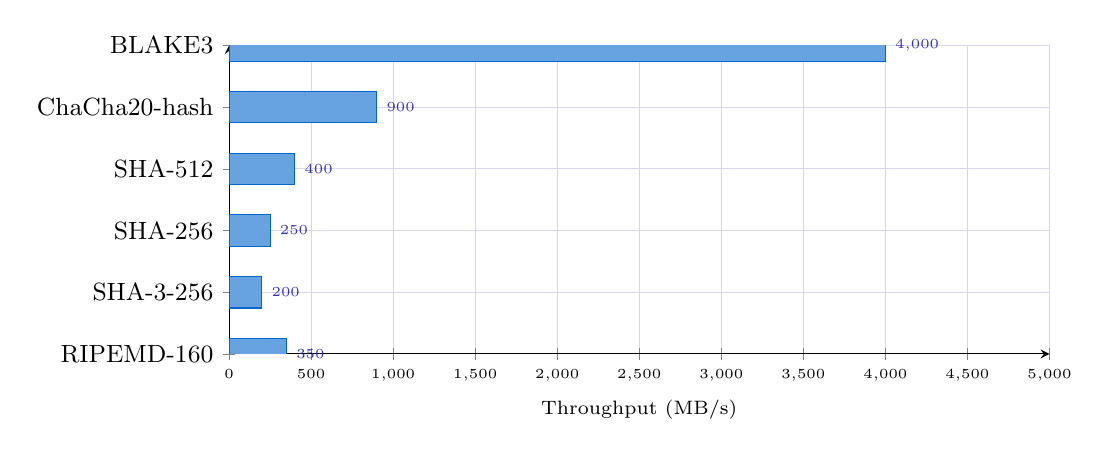
\begin{tikzpicture}
\begin{axis}[
  xbar,
  width=12cm, height=5.5cm,
  xlabel={\scriptsize Throughput (MB/s)},
  symbolic y coords={RIPEMD-160,SHA-3-256,SHA-256,SHA-512,ChaCha20-hash,BLAKE3},
  ytick=data,
  y tick label style={font=\small},
  x tick label style={font=\tiny},
  xmin=0, xmax=5000,
  nodes near coords,
  nodes near coords style={font=\tiny,mlpurple},
  bar width=0.4cm,
  axis lines=left,
  grid=major,
  grid style={mllavender4},
  xlabel style={font=\scriptsize},
]
\addplot[fill=mlblue!60,draw=mlblue] coordinates {
  (350,RIPEMD-160)
  (200,SHA-3-256)
  (250,SHA-256)
  (400,SHA-512)
  (900,ChaCha20-hash)
  (4000,BLAKE3)
};
\end{axis}
\end{tikzpicture}
\end{center}
\vspace{1mm}
\begin{columns}
\column{0.48\textwidth}
\begin{block}{Key Observations}
\begin{itemize}\small
  \item \textbf{BLAKE3}: tree-hashing parallelism $\to$ $\sim$16$\times$ SHA-256
  \item \textbf{SHA-512}: faster than SHA-256 on 64-bit CPUs
  \item \textbf{SHA-3}: secure but slower in software (fast in hardware)
\end{itemize}
\end{block}
\column{0.48\textwidth}
\begin{block}{Blockchain Usage}
\begin{itemize}\small
  \item Bitcoin: SHA-256d (double hash)
  \item Ethereum: Keccak-256 (pre-NIST SHA-3 variant)
  \item Zcash: BLAKE2b for Equihash PoW
  \item Addresses: RIPEMD-160(SHA-256(pubkey))
\end{itemize}
\end{block}
\end{columns}
\bottomnote{Benchmarks: single-core, x86-64, 1 KiB messages; BLAKE3 exploits SIMD and tree parallelism}
\end{frame}

%--- FRAME 12: Hash Applications in Blockchain ---
\begin{frame}{Hash Applications in Blockchain}
\begin{center}
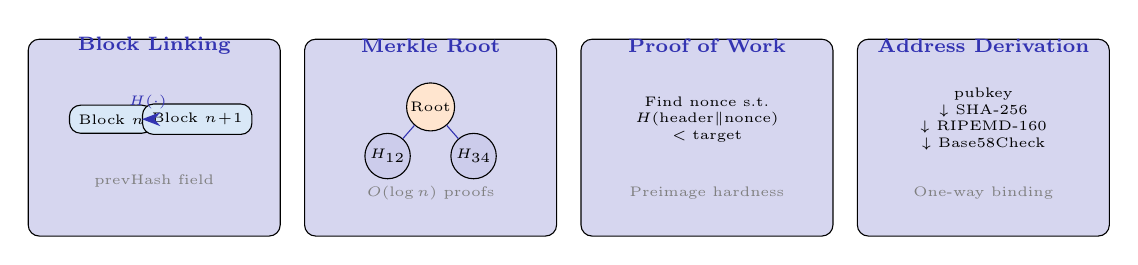
\begin{tikzpicture}[scale=0.78,
  panel/.style={draw,rounded corners,fill=mllavender4,minimum width=3.2cm,minimum height=2.5cm,align=center},
  label/.style={font=\scriptsize\bfseries,mlpurple}]
  % Panel 1: Block Linking
  \node[panel] (p1) at (0,0) {};
  \node[label] at (0,1.5) {Block Linking};
  \node[draw,fill=mlblue!15,rounded corners,font=\tiny,minimum width=1cm] (b1) at (-0.7,0.3) {Block $n$};
  \node[draw,fill=mlblue!15,rounded corners,font=\tiny,minimum width=1cm] (b2) at (0.7,0.3) {Block $n\!+\!1$};
  \draw[-{Stealth},mlpurple,thick] (b1) -- (b2) node[midway,above,font=\tiny]{$H(\cdot)$};
  \node[font=\tiny,mlgray] at (0,-0.7) {prevHash field};
  % Panel 2: Merkle Root
  \node[panel] (p2) at (4.5,0) {};
  \node[label] at (4.5,1.5) {Merkle Root};
  \node[draw,circle,fill=mlorange!20,inner sep=1pt,font=\tiny] (root) at (4.5,0.5) {Root};
  \node[draw,circle,fill=mllavender3,inner sep=1pt,font=\tiny] (h1) at (3.8,-0.3) {$H_{12}$};
  \node[draw,circle,fill=mllavender3,inner sep=1pt,font=\tiny] (h2) at (5.2,-0.3) {$H_{34}$};
  \draw[mlpurple] (root)--(h1); \draw[mlpurple] (root)--(h2);
  \node[font=\tiny,mlgray] at (4.5,-0.9) {$O(\log n)$ proofs};
  % Panel 3: Proof of Work
  \node[panel] (p3) at (9.0,0) {};
  \node[label] at (9.0,1.5) {Proof of Work};
  \node[font=\tiny,align=center] at (9.0,0.3) {Find nonce s.t.\\$H(\text{header} \| \text{nonce})$\\$< \text{target}$};
  \node[font=\tiny,mlgray] at (9.0,-0.9) {Preimage hardness};
  % Panel 4: Address Derivation
  \node[panel] (p4) at (13.5,0) {};
  \node[label] at (13.5,1.5) {Address Derivation};
  \node[font=\tiny,align=center] at (13.5,0.3) {pubkey\\$\downarrow$ SHA-256\\$\downarrow$ RIPEMD-160\\$\downarrow$ Base58Check};
  \node[font=\tiny,mlgray] at (13.5,-0.9) {One-way binding};
\end{tikzpicture}
\end{center}
\vspace{2mm}
\begin{columns}
\column{0.48\textwidth}
\begin{block}{Why Hash Functions Are Fundamental}
\begin{itemize}\small
  \item \textbf{Integrity}: any change invalidates the chain
  \item \textbf{Commitment}: miners commit to block content
  \item \textbf{Efficiency}: Merkle proofs enable light clients
\end{itemize}
\end{block}
\column{0.48\textwidth}
\begin{block}{Hash Count per Bitcoin Block}
\begin{itemize}\small
  \item Block header hash: 2$\times$ SHA-256
  \item Merkle tree: $\sim 2N-1$ hashes for $N$ txs
  \item Addresses: SHA-256 + RIPEMD-160 each
  \item PoW: billions of trial hashes per second
\end{itemize}
\end{block}
\end{columns}
\bottomnote{Hash functions are the most-used cryptographic primitive in any blockchain system}
\end{frame}

\section{Symmetric Cryptography}

%--- FRAME 13: Symmetric Encryption Formal ---
\begin{frame}{Symmetric Encryption: Formal Definitions}
\begin{block}{Definition}
A symmetric encryption scheme is a triple $(\mathcal{K}, \mathcal{E}, \mathcal{D})$ over key space $\mathbb{K}$, message space $\mathbb{M}$, ciphertext space $\mathbb{C}$:
\[
  \mathcal{E}_k : \mathbb{M} \to \mathbb{C}, \qquad \mathcal{D}_k : \mathbb{C} \to \mathbb{M}, \qquad \forall\, m \in \mathbb{M},\; k \in \mathbb{K}:\; \mathcal{D}_k(\mathcal{E}_k(m)) = m
\]
\end{block}
\vspace{1mm}
\begin{columns}
\column{0.48\textwidth}
\begin{block}{Security Notion: IND-CPA}
\small An adversary $\mathcal{A}$ with access to encryption oracle $\mathcal{E}_k(\cdot)$ picks $(m_0, m_1)$, receives $c^* = \mathcal{E}_k(m_b)$ for random $b$, and guesses $b$. The scheme is IND-CPA secure if:
\[
  \left|\Pr[\mathcal{A} \text{ wins}] - \tfrac{1}{2}\right| \leq \text{negl}(\lambda)
\]
\end{block}
\column{0.48\textwidth}
\begin{block}{Key Properties}
\begin{itemize}\small
  \item \textbf{Same key} for encryption and decryption
  \item Key must be shared via \textbf{secure channel}
  \item For $n$ parties: $\binom{n}{2} = \frac{n(n-1)}{2}$ keys needed
  \item Very fast: hardware AES-NI $\sim$ 1 GB/s
\end{itemize}
\end{block}
\vspace{1mm}
\begin{block}{Blockchain Relevance}
\begin{itemize}\small
  \item Encrypted wallet files (AES-256-CBC)
  \item Secure P2P channels (AES-GCM in TLS)
  \item BIP-38 passphrase-protected private keys
\end{itemize}
\end{block}
\end{columns}
\bottomnote{Symmetric crypto is $\sim\!1000\times$ faster than asymmetric -- used for bulk data, not authentication}
\end{frame}

%--- FRAME 14: AES Overview ---
\begin{frame}{AES Round Structure}
\begin{center}
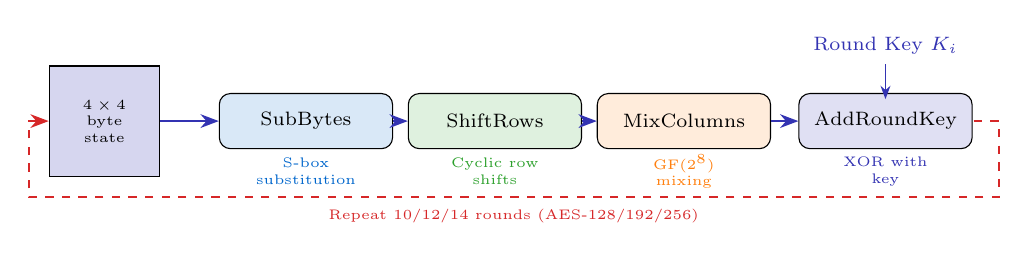
\begin{tikzpicture}[scale=0.8,
  procstep/.style={draw,rounded corners,minimum width=2.2cm,minimum height=0.7cm,font=\scriptsize},
  mat/.style={draw,fill=mllavender4,minimum width=1.4cm,minimum height=1.4cm,font=\tiny,align=center}]
  % 4x4 state matrix
  \node[mat] (state) at (0,0) {$4 \times 4$\\byte\\state};
  % Steps
  \node[procstep,fill=mlblue!15] (sub) at (3.2,0) {SubBytes};
  \node[procstep,fill=mlgreen!15] (shift) at (6.2,0) {ShiftRows};
  \node[procstep,fill=mlorange!15] (mix) at (9.2,0) {MixColumns};
  \node[procstep,fill=mlpurple!15] (add) at (12.4,0) {AddRoundKey};
  % Arrows
  \draw[-{Stealth},thick,mlpurple] (state) -- (sub);
  \draw[-{Stealth},thick,mlpurple] (sub) -- (shift);
  \draw[-{Stealth},thick,mlpurple] (shift) -- (mix);
  \draw[-{Stealth},thick,mlpurple] (mix) -- (add);
  % Round key input
  \node[font=\scriptsize,mlpurple] at (12.4,1.2) {Round Key $K_i$};
  \draw[-{Stealth},mlpurple] (12.4,0.9) -- (12.4,0.35);
  % Loop arrow
  \draw[-{Stealth},thick,mlred,dashed] (13.8,0) -- (14.2,0) -- (14.2,-1.2) -- (-1.2,-1.2) -- (-1.2,0) -- (state);
  \node[font=\tiny,mlred] at (6.5,-1.5) {Repeat 10/12/14 rounds (AES-128/192/256)};
  % Step descriptions
  \node[font=\tiny,mlblue,align=center] at (3.2,-0.8) {S-box\\substitution};
  \node[font=\tiny,mlgreen,align=center] at (6.2,-0.8) {Cyclic row\\shifts};
  \node[font=\tiny,mlorange,align=center] at (9.2,-0.8) {GF($2^8$)\\mixing};
  \node[font=\tiny,mlpurple,align=center] at (12.4,-0.8) {XOR with\\key};
\end{tikzpicture}
\end{center}
\vspace{2mm}
\begin{columns}
\column{0.48\textwidth}
\begin{block}{Design Principles}
\begin{itemize}\small
  \item \textbf{Confusion}: SubBytes (non-linear S-box in $\text{GF}(2^8)$)
  \item \textbf{Diffusion}: ShiftRows + MixColumns spread influence
  \item \textbf{Key mixing}: AddRoundKey via XOR
  \item Full diffusion after 2 rounds; 10+ for security margin
\end{itemize}
\end{block}
\column{0.48\textwidth}
\begin{block}{AES Variants}
\small
\begin{tabular}{lccc}
\toprule
& \textbf{128} & \textbf{192} & \textbf{256} \\
\midrule
Key bits & 128 & 192 & 256 \\
Rounds & 10 & 12 & 14 \\
Security & 128 & 192 & 256 \\
\bottomrule
\end{tabular}
\vspace{2mm}\\
\scriptsize Best known attack: biclique -- reduces AES-256 to $2^{254.4}$ (still impractical).
\end{block}
\end{columns}
\bottomnote{AES (Rijndael) standardized by NIST in 2001; ubiquitous in TLS, disk encryption, and wallet protection}
\end{frame}

%--- FRAME 15: Block Cipher Modes ---
\begin{frame}{Block Cipher Modes of Operation}
\begin{center}
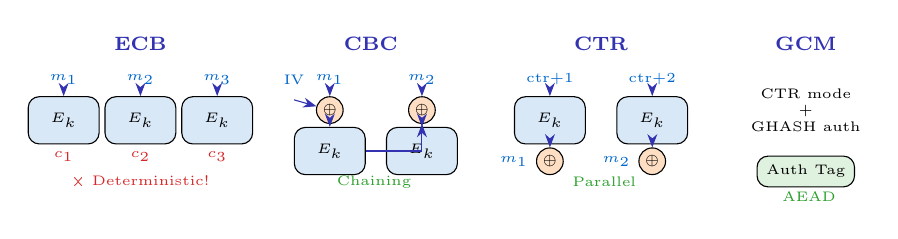
\begin{tikzpicture}[scale=0.65,
  block/.style={draw,rounded corners,fill=mlblue!15,minimum width=0.9cm,minimum height=0.6cm,font=\tiny\bfseries},
  xornode/.style={draw,circle,fill=mlorange!25,inner sep=1pt,font=\tiny},
  msg/.style={font=\tiny,mlblue}]
  % ECB
  \node[font=\scriptsize\bfseries,mlpurple] at (1.5,2.5) {ECB};
  \node[msg] at (0,1.8) {$m_1$};
  \node[msg] at (1.5,1.8) {$m_2$};
  \node[msg] at (3.0,1.8) {$m_3$};
  \node[block] (ecb1) at (0,1.0) {$E_k$};
  \node[block] (ecb2) at (1.5,1.0) {$E_k$};
  \node[block] (ecb3) at (3.0,1.0) {$E_k$};
  \draw[-{Stealth},mlpurple] (0,1.6)--(ecb1); \draw[-{Stealth},mlpurple] (1.5,1.6)--(ecb2); \draw[-{Stealth},mlpurple] (3.0,1.6)--(ecb3);
  \node[font=\tiny,mlred] at (0,0.3) {$c_1$}; \node[font=\tiny,mlred] at (1.5,0.3) {$c_2$}; \node[font=\tiny,mlred] at (3.0,0.3) {$c_3$};
  \node[font=\tiny,mlred] at (1.5,-0.2) {\texttimes\ Deterministic!};

  % CBC
  \node[font=\scriptsize\bfseries,mlpurple] at (6.0,2.5) {CBC};
  \node[msg] at (4.5,1.8) {IV};
  \node[msg] at (5.2,1.8) {$m_1$};
  \node[msg] at (7.0,1.8) {$m_2$};
  \node[xornode] (cbcx1) at (5.2,1.2) {$\oplus$};
  \node[block] (cbc1) at (5.2,0.4) {$E_k$};
  \node[xornode] (cbcx2) at (7.0,1.2) {$\oplus$};
  \node[block] (cbc2) at (7.0,0.4) {$E_k$};
  \draw[-{Stealth},mlpurple] (5.2,1.6)--(cbcx1); \draw[-{Stealth},mlpurple] (cbcx1)--(cbc1);
  \draw[-{Stealth},mlpurple] (4.5,1.4)--(cbcx1);
  \draw[-{Stealth},mlpurple] (cbc1.east) -| (cbcx2);
  \draw[-{Stealth},mlpurple] (7.0,1.6)--(cbcx2); \draw[-{Stealth},mlpurple] (cbcx2)--(cbc2);
  \node[font=\tiny,mlgreen] at (6.0,-0.2) {\checkmark\ Chaining};

  % CTR
  \node[font=\scriptsize\bfseries,mlpurple] at (10.5,2.5) {CTR};
  \node[msg] at (9.5,1.8) {ctr+1};
  \node[msg] at (11.5,1.8) {ctr+2};
  \node[block] (ctr1) at (9.5,1.0) {$E_k$};
  \node[block] (ctr2) at (11.5,1.0) {$E_k$};
  \draw[-{Stealth},mlpurple] (9.5,1.6)--(ctr1); \draw[-{Stealth},mlpurple] (11.5,1.6)--(ctr2);
  \node[xornode] (ctrx1) at (9.5,0.2) {$\oplus$};
  \node[xornode] (ctrx2) at (11.5,0.2) {$\oplus$};
  \draw[-{Stealth},mlpurple] (ctr1)--(ctrx1); \draw[-{Stealth},mlpurple] (ctr2)--(ctrx2);
  \node[font=\tiny,mlblue] at (8.8,0.2) {$m_1$}; \node[font=\tiny,mlblue] at (10.8,0.2) {$m_2$};
  \node[font=\tiny,mlgreen] at (10.5,-0.2) {\checkmark\ Parallel};

  % GCM
  \node[font=\scriptsize\bfseries,mlpurple] at (14.5,2.5) {GCM};
  \node[font=\tiny,align=center] at (14.5,1.2) {CTR mode\\+\\GHASH auth};
  \node[draw,rounded corners,fill=mlgreen!15,font=\tiny] at (14.5,0) {Auth Tag};
  \node[font=\tiny,mlgreen] at (14.5,-0.5) {\checkmark\ AEAD};
\end{tikzpicture}
\end{center}
\vspace{2mm}
\begin{columns}
\column{0.48\textwidth}
\begin{block}{Mode Comparison}
\scriptsize
\begin{tabular}{lcccc}
\toprule
 & \textbf{ECB} & \textbf{CBC} & \textbf{CTR} & \textbf{GCM} \\
\midrule
IND-CPA & \textcolor{mlred}{\texttimes} & \checkmark & \checkmark & \checkmark \\
Parallel enc & \checkmark & \textcolor{mlred}{\texttimes} & \checkmark & \checkmark \\
Auth (AEAD) & \textcolor{mlred}{\texttimes} & \textcolor{mlred}{\texttimes} & \textcolor{mlred}{\texttimes} & \checkmark \\
\bottomrule
\end{tabular}
\end{block}
\column{0.48\textwidth}
\begin{block}{Blockchain Usage}
\begin{itemize}\small
  \item \textbf{AES-256-CBC}: Bitcoin Core wallet encryption
  \item \textbf{AES-GCM}: TLS 1.3 for P2P node communication
  \item \textbf{CTR mode}: Preferred for parallelism in hardware wallets
  \item Never use ECB for any security-sensitive application
\end{itemize}
\end{block}
\end{columns}
\bottomnote{GCM (Galois/Counter Mode) provides both confidentiality and integrity -- the modern standard for AEAD}
\end{frame}

%--- FRAME 16: Diffie-Hellman Key Exchange ---
\begin{frame}{Diffie--Hellman Key Exchange}
\begin{center}
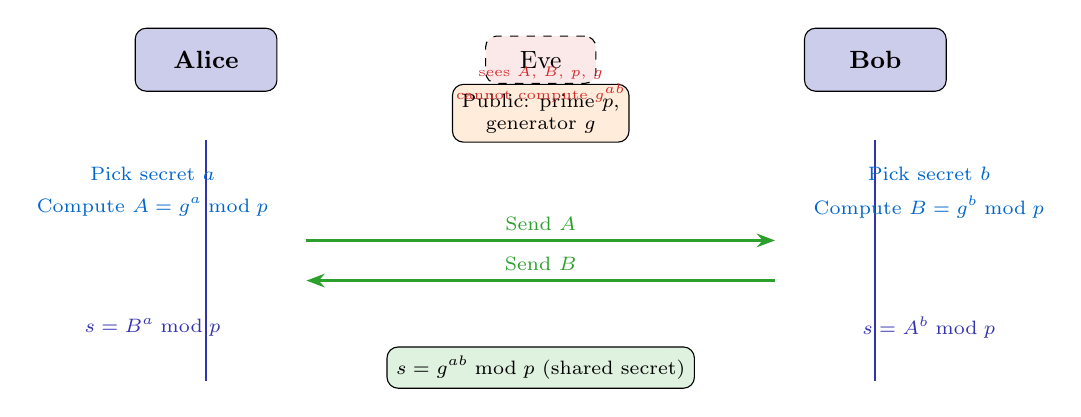
\begin{tikzpicture}[scale=0.85,
  person/.style={draw,rounded corners,fill=mllavender3,minimum width=1.8cm,minimum height=0.8cm,font=\small\bfseries}]
  % Actors
  \node[person] (alice) at (0,5) {Alice};
  \node[person] (bob) at (10,5) {Bob};
  \node[draw,dashed,rounded corners,fill=mlred!10,minimum width=1.4cm,minimum height=0.6cm,font=\small] (eve) at (5,5) {Eve};
  % Public parameters
  \node[draw,rounded corners,fill=mlorange!15,font=\scriptsize,align=center] at (5,4.2) {Public: prime $p$,\\generator $g$};
  % Vertical lines
  \draw[mlpurple,thick] (0,3.8) -- (0,0.2);
  \draw[mlpurple,thick] (10,3.8) -- (10,0.2);
  % Alice picks secret
  \node[font=\scriptsize,mlblue,align=left] at (-0.8,3.3) {Pick secret $a$};
  \node[font=\scriptsize,mlblue,align=left] at (-0.8,2.8) {Compute $A = g^a \bmod p$};
  % Bob picks secret
  \node[font=\scriptsize,mlblue,align=right] at (10.8,3.3) {Pick secret $b$};
  \node[font=\scriptsize,mlblue,align=right] at (10.8,2.8) {Compute $B = g^b \bmod p$};
  % Exchange
  \draw[-{Stealth},thick,mlgreen] (1.5,2.3) -- (8.5,2.3) node[midway,above,font=\scriptsize]{Send $A$};
  \draw[-{Stealth},thick,mlgreen] (8.5,1.7) -- (1.5,1.7) node[midway,above,font=\scriptsize]{Send $B$};
  % Shared secret
  \node[font=\scriptsize,mlpurple,align=left] at (-0.8,1.0) {$s = B^a \bmod p$};
  \node[font=\scriptsize,mlpurple,align=right] at (10.8,1.0) {$s = A^b \bmod p$};
  % Result
  \node[draw,rounded corners,fill=mlgreen!15,font=\scriptsize] at (5,0.4) {$s = g^{ab} \bmod p$ (shared secret)};
  % Eve label
  \node[font=\tiny,mlred] at (5,4.8) {sees $A$, $B$, $p$, $g$};
  \node[font=\tiny,mlred] at (5,4.5) {cannot compute $g^{ab}$};
\end{tikzpicture}
\end{center}
\vspace{1mm}
\begin{columns}
\column{0.48\textwidth}
\begin{block}{Security Basis}
\small \textbf{Decisional Diffie--Hellman (DDH):}\\
Given $(g, g^a, g^b)$, it is hard to distinguish $g^{ab}$ from $g^c$ for random $c$.
\end{block}
\column{0.48\textwidth}
\begin{block}{Limitations}
\begin{itemize}\small
  \item Vulnerable to \textbf{man-in-the-middle} without authentication
  \item No identity verification -- must combine with signatures
  \item Basis for ECDH (Elliptic Curve DH) used in modern TLS
\end{itemize}
\end{block}
\end{columns}
\bottomnote{Diffie \& Hellman (1976): first published public-key protocol; foundation of modern key exchange}
\end{frame}

%--- FRAME 17: Symmetric vs Asymmetric Trade-offs ---
\begin{frame}{Symmetric vs.\ Asymmetric: Performance Trade-offs}
\begin{center}
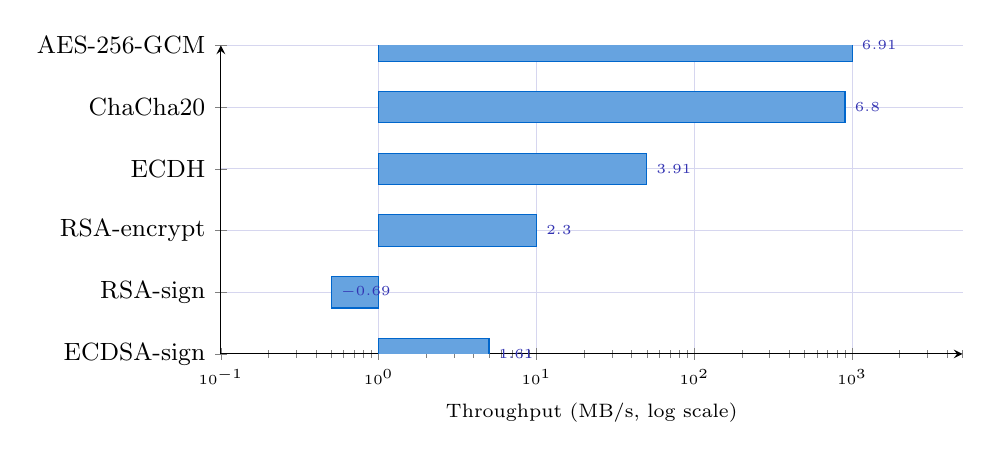
\begin{tikzpicture}
\begin{axis}[
  xbar,
  width=11cm, height=5.5cm,
  xlabel={\scriptsize Throughput (MB/s, log scale)},
  xmode=log,
  symbolic y coords={ECDSA-sign,RSA-sign,RSA-encrypt,ECDH,ChaCha20,AES-256-GCM},
  ytick=data,
  y tick label style={font=\small},
  x tick label style={font=\tiny},
  xmin=0.1, xmax=5000,
  nodes near coords,
  nodes near coords style={font=\tiny,mlpurple,anchor=west},
  bar width=0.4cm,
  axis lines=left,
  grid=major,
  grid style={mllavender4},
  xlabel style={font=\scriptsize},
]
\addplot[fill=mlblue!60,draw=mlblue] coordinates {
  (5,ECDSA-sign)
  (0.5,RSA-sign)
  (10,RSA-encrypt)
  (50,ECDH)
  (900,ChaCha20)
  (1000,AES-256-GCM)
};
\end{axis}
\end{tikzpicture}
\end{center}
\vspace{1mm}
\begin{columns}
\column{0.48\textwidth}
\begin{block}{Symmetric Advantages}
\begin{itemize}\small
  \item $100$--$1000\times$ faster than asymmetric
  \item Constant-time implementations easier
  \item Hardware acceleration (AES-NI, ARM CE)
  \item Used for bulk encryption after key exchange
\end{itemize}
\end{block}
\column{0.48\textwidth}
\begin{block}{Asymmetric Advantages}
\begin{itemize}\small
  \item No pre-shared secret required
  \item Digital signatures for authentication
  \item Key distribution scales: $n$ keys for $n$ parties
  \item Non-repudiation (signatures prove origin)
\end{itemize}
\end{block}
\end{columns}
\bottomnote{Hybrid approach: asymmetric crypto for key exchange, symmetric for data -- best of both worlds}
\end{frame}

\section{Asymmetric Cryptography}

%--- FRAME 18: RSA Mathematics ---
\begin{frame}{RSA: Mathematical Foundations}
\begin{block}{Key Generation}
\begin{enumerate}\small
  \item Choose two large primes $p, q$ (each $\geq 1024$ bits)
  \item Compute $n = p \cdot q$ \quad and \quad $\phi(n) = (p-1)(q-1)$
  \item Choose $e$ with $\gcd(e, \phi(n)) = 1$ \quad (common: $e = 65537$)
  \item Compute $d \equiv e^{-1} \pmod{\phi(n)}$ \quad (extended Euclidean algorithm)
  \item Public key: $(n, e)$ \qquad Private key: $(n, d)$
\end{enumerate}
\end{block}
\vspace{1mm}
\begin{columns}
\column{0.48\textwidth}
\begin{block}{Encryption / Decryption}
\begin{align*}
  \text{Encrypt:} \quad c &= m^e \bmod n \\
  \text{Decrypt:} \quad m &= c^d \bmod n
\end{align*}
\textbf{Correctness:} By Euler's theorem,
\[
  c^d = m^{ed} = m^{1 + k\phi(n)} = m \cdot (m^{\phi(n)})^k \equiv m \pmod{n}
\]
\end{block}
\column{0.48\textwidth}
\begin{block}{Security Assumptions}
\begin{itemize}\small
  \item \textbf{RSA problem}: Given $c = m^e \bmod n$, find $m$
  \item \textbf{Factoring}: Given $n = pq$, find $p, q$
  \item Best known: General Number Field Sieve
    \[
      L_n\!\left[\tfrac{1}{3},\, 1.923\right] = e^{1.923(\ln n)^{1/3}(\ln \ln n)^{2/3}}
    \]
  \item RSA-2048: $\sim 2^{112}$ security (sub-exponential)
\end{itemize}
\end{block}
\end{columns}
\vspace{1mm}
\begin{alertblock}{Why Blockchain Doesn't Use RSA}
\small RSA-2048 keys are 256 bytes vs.\ ECDSA-256 keys at 32 bytes. RSA signatures are $\sim$50$\times$ larger and $\sim$10$\times$ slower. ECC provides equivalent security with far smaller keys.
\end{alertblock}
\bottomnote{RSA (Rivest--Shamir--Adleman, 1978): foundational but largely superseded by ECC in blockchain}
\end{frame}

%--- FRAME 19: Elliptic Curve Fundamentals ---
\begin{frame}{Elliptic Curve Fundamentals}
\begin{columns}
\column{0.42\textwidth}
\begin{center}
\begin{tikzpicture}[scale=0.85]
\begin{axis}[
  width=6cm, height=6cm,
  axis lines=middle,
  xlabel={$x$}, ylabel={$y$},
  xlabel style={font=\tiny,at={(1,0.48)}},
  ylabel style={font=\tiny,at={(0.48,1)}},
  xmin=-2, xmax=4,
  ymin=-4, ymax=4,
  ticks=none,
  clip=false,
  axis line style={mlgray}
]
% Curve: y^2 = x^3 - 3x + 5 (smooth real curve)
\addplot[mlpurple,thick,domain=-1.45:3.5,samples=200,smooth] {sqrt(x^3 - 3*x + 5)};
\addplot[mlpurple,thick,domain=-1.45:3.5,samples=200,smooth] {-sqrt(x^3 - 3*x + 5)};
% Point P
\addplot[only marks,mark=*,mlblue,mark size=2pt] coordinates {(0,2.236)};
\node[font=\scriptsize,mlblue,above right] at (axis cs:0,2.236) {$P$};
% Point Q
\addplot[only marks,mark=*,mlgreen,mark size=2pt] coordinates {(2,2.646)};
\node[font=\scriptsize,mlgreen,above right] at (axis cs:2,2.646) {$Q$};
% Line through P and Q
\addplot[mlred,dashed,thin,domain=-1.5:3.5] {2.236 + 0.205*(x-0)};
% Intersection point R'
\addplot[only marks,mark=*,mlgray,mark size=2pt] coordinates {(3.13,2.878)};
\node[font=\scriptsize,mlgray,above] at (axis cs:3.13,2.878) {$R'$};
% Reflected point R = P+Q
\addplot[only marks,mark=*,mlorange,mark size=2pt] coordinates {(3.13,-2.878)};
\node[font=\scriptsize,mlorange,below right] at (axis cs:3.13,-2.878) {$R=P+Q$};
% Vertical reflection line
\draw[mlgray,dotted] (axis cs:3.13,2.878) -- (axis cs:3.13,-2.878);
\end{axis}
\end{tikzpicture}
\end{center}
\column{0.55\textwidth}
\begin{block}{Weierstrass Form}
\[
  y^2 = x^3 + ax + b, \qquad 4a^3 + 27b^2 \neq 0 \;\text{(non-singular)}
\]
\end{block}
\vspace{1mm}
\begin{block}{Point Addition (Geometric)}
\begin{enumerate}\small
  \item Draw line through $P$ and $Q$
  \item Find third intersection $R'$ with the curve
  \item Reflect $R'$ across $x$-axis: $R = P + Q$
\end{enumerate}
\end{block}
\vspace{1mm}
\begin{block}{Algebraic Formulas}
\small For $P=(x_1,y_1)$, $Q=(x_2,y_2)$, $P \neq Q$:
\begin{align*}
  \lambda &= \frac{y_2 - y_1}{x_2 - x_1}, \\
  x_3 &= \lambda^2 - x_1 - x_2, \\
  y_3 &= \lambda(x_1 - x_3) - y_1
\end{align*}
Point at infinity $\mathcal{O}$ serves as identity.
\end{block}
\end{columns}
\bottomnote{Elliptic curves over finite fields form an abelian group -- the foundation of ECC}
\end{frame}

%--- FRAME 20: ECDSA Key Generation ---
\begin{frame}{ECDSA Key Generation \& secp256k1 Parameters}
\begin{columns}
\column{0.48\textwidth}
\begin{block}{secp256k1 Parameters (Bitcoin)}
\scriptsize
\begin{tabular}{lp{5.5cm}}
\toprule
\textbf{Parameter} & \textbf{Value} \\
\midrule
Curve & $y^2 = x^3 + 7$ over $\mathbb{F}_p$ \\
$p$ & $2^{256} - 2^{32} - 977$ \\
$a$ & $0$ \\
$b$ & $7$ \\
$G$ (generator) & Specified 256-bit $(x,y)$ point \\
$n$ (order) & $\approx 2^{256}$ (exact 256-bit prime) \\
$h$ (cofactor) & $1$ \\
\bottomrule
\end{tabular}
\end{block}
\vspace{1mm}
\begin{alertblock}{Why secp256k1?}
\small Koblitz curve: no suspicious constants (``nothing up my sleeve''), efficient endomorphism for $\sim 30\%$ speedup.
\end{alertblock}
\column{0.48\textwidth}
\begin{block}{Key Generation Algorithm}
\begin{enumerate}\small
  \item Select random $d \in [1, n-1]$ \\ (private key: 256-bit integer)
  \item Compute $Q = d \cdot G$ \\ (public key: point on curve)
  \item Verify $Q \neq \mathcal{O}$ and $Q$ is on the curve
\end{enumerate}
\end{block}
\vspace{1mm}
\begin{block}{Security Guarantee}
\small Given $Q = dG$, finding $d$ requires solving the \textbf{Elliptic Curve Discrete Logarithm Problem (ECDLP)}.\\[2mm]
Best known attack: Pollard's rho\\
Complexity: $\mathcal{O}(\sqrt{n}) \approx 2^{128}$ operations\\[2mm]
\textbf{Key sizes for 128-bit security:}\\
$\bullet$ RSA: 3072 bits \quad $\bullet$ ECC: 256 bits
\end{block}
\end{columns}
\bottomnote{ECDSA private key = 32 bytes; public key = 33 bytes (compressed) -- compact enough for every transaction}
\end{frame}

%--- FRAME 21: Discrete Logarithm Problem ---
\begin{frame}{Attack Complexity: RSA vs.\ ECDLP}
\begin{center}
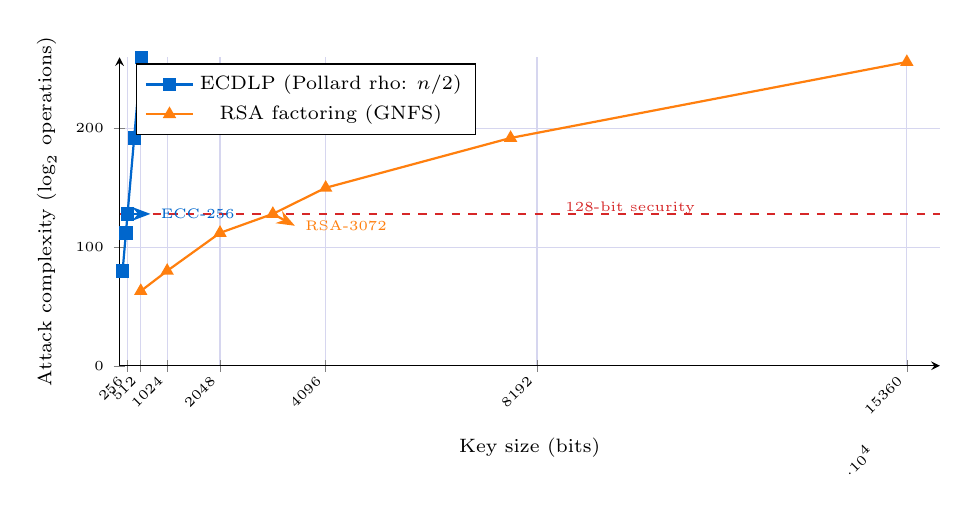
\begin{tikzpicture}
\begin{axis}[
  width=12cm, height=5.5cm,
  xlabel={\scriptsize Key size (bits)},
  ylabel={\scriptsize Attack complexity ($\log_2$ operations)},
  xmin=100, xmax=16000,
  ymin=0, ymax=260,
  grid=major,
  grid style={mllavender4},
  axis lines=left,
  xlabel style={font=\scriptsize},
  ylabel style={font=\scriptsize},
  tick label style={font=\tiny},
  legend style={font=\scriptsize,at={(0.02,0.98)},anchor=north west},
  xtick={256,512,1024,2048,4096,8192,15360},
  xticklabels={256,512,1024,2048,4096,8192,15360},
  x tick label style={rotate=45,anchor=east,font=\tiny},
]
% ECDLP: sqrt(n) -> key/2 bits of security
\addplot[mlblue,thick,mark=square*,mark size=2pt] coordinates {
  (160,80) (224,112) (256,128) (384,192) (521,260)
};
\addlegendentry{ECDLP (Pollard rho: $n/2$)}
% RSA: sub-exponential GNFS
\addplot[mlorange,thick,mark=triangle*,mark size=2pt] coordinates {
  (512,63) (1024,80) (2048,112) (3072,128) (4096,150) (7680,192) (15360,256)
};
\addlegendentry{RSA factoring (GNFS)}
% 128-bit security line
\draw[mlred,dashed,thick] (axis cs:100,128) -- (axis cs:16000,128);
\node[font=\tiny,mlred] at (axis cs:10000,133) {128-bit security};
% Annotations
\draw[-{Stealth},mlblue,thick] (axis cs:256,128) -- (axis cs:700,128) node[right,font=\tiny,mlblue]{ECC-256};
\draw[-{Stealth},mlorange,thick] (axis cs:3072,128) -- (axis cs:3500,118) node[right,font=\tiny,mlorange]{RSA-3072};
\end{axis}
\end{tikzpicture}
\end{center}
\vspace{1mm}
\begin{columns}
\column{0.48\textwidth}
\begin{block}{ECDLP Hardness}
\begin{itemize}\small
  \item Best generic attack: $\mathcal{O}(\sqrt{n})$ (Pollard rho)
  \item No sub-exponential algorithm known
  \item 256-bit key $\to$ $2^{128}$ security
\end{itemize}
\end{block}
\column{0.48\textwidth}
\begin{block}{RSA Factoring}
\begin{itemize}\small
  \item GNFS: sub-exponential $L[1/3, 1.923]$
  \item 3072-bit key $\to$ $2^{128}$ security
  \item $12\times$ larger key for same security level
\end{itemize}
\end{block}
\end{columns}
\bottomnote{ECC achieves equivalent security with $\sim$12$\times$ smaller keys -- critical for blockchain transaction size}
\end{frame}

%--- FRAME 22: Ed25519 & Curve25519 ---
\begin{frame}{Ed25519 \& Curve25519}
\begin{block}{Modern Elliptic Curve Designs (Bernstein et al.)}
\small Two complementary curves from the same mathematical family, optimized for different uses.
\end{block}
\vspace{2mm}
\begin{center}
\small
\begin{tabular}{lll}
\toprule
\textbf{Property} & \textbf{Ed25519 (EdDSA)} & \textbf{Curve25519 (X25519)} \\
\midrule
Primary use & Digital signatures & Key exchange (ECDH) \\
Curve form & Twisted Edwards: $-x^2+y^2=1+dx^2y^2$ & Montgomery: $y^2=x^3+486662x^2+x$ \\
Field prime & $p = 2^{255} - 19$ & $p = 2^{255} - 19$ \\
Security level & $\sim 128$ bits & $\sim 128$ bits \\
Signature size & 64 bytes & -- \\
Public key size & 32 bytes & 32 bytes \\
Deterministic nonce & Yes (RFC 8032) & -- \\
Constant-time & By design & By design \\
Side-channel safe & Yes & Yes \\
\bottomrule
\end{tabular}
\end{center}
\vspace{2mm}
\begin{columns}
\column{0.48\textwidth}
\begin{block}{Advantages over secp256k1}
\begin{itemize}\small
  \item \textbf{Deterministic}: no random nonce $\to$ no nonce-reuse vulnerability
  \item \textbf{Faster}: $\sim 3\times$ signature verification speed
  \item \textbf{Complete formulas}: no edge cases in point addition
\end{itemize}
\end{block}
\column{0.48\textwidth}
\begin{block}{Adoption}
\begin{itemize}\small
  \item Solana, Cardano, Polkadot: Ed25519
  \item Signal Protocol, WireGuard: X25519/Ed25519
  \item SSH, TLS 1.3: Ed25519 supported
  \item Bitcoin: still secp256k1 (network effect)
\end{itemize}
\end{block}
\end{columns}
\bottomnote{Ed25519 eliminates the most dangerous implementation pitfall of ECDSA: random nonce generation}
\end{frame}

%--- FRAME 23: EC Point Multiplication ---
\begin{frame}{EC Point Multiplication: Double-and-Add}
\begin{columns}
\column{0.52\textwidth}
\begin{center}
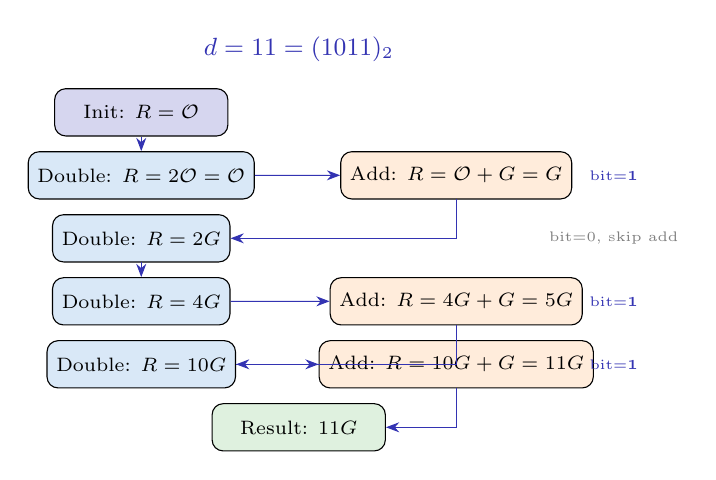
\begin{tikzpicture}[scale=0.8,
  procstep/.style={draw,rounded corners,minimum width=2.2cm,minimum height=0.6cm,font=\scriptsize,align=center},
  result/.style={draw,rounded corners,fill=mlgreen!15,minimum width=2.2cm,minimum height=0.6cm,font=\scriptsize}]
  % Title
  \node[font=\small\bfseries,mlpurple] at (2.5,5.5) {$d = 11 = (1011)_2$};
  % Steps
  \node[procstep,fill=mllavender4] (s0) at (0,4.5) {Init: $R = \mathcal{O}$};
  % Bit 3 (MSB) = 1
  \node[procstep,fill=mlblue!15] (s1a) at (0,3.5) {Double: $R = 2\mathcal{O} = \mathcal{O}$};
  \node[procstep,fill=mlorange!15] (s1b) at (5,3.5) {Add: $R = \mathcal{O}+G = G$};
  \node[font=\tiny,mlpurple] at (7.5,3.5) {bit=\textbf{1}};
  % Bit 2 = 0
  \node[procstep,fill=mlblue!15] (s2a) at (0,2.5) {Double: $R = 2G$};
  \node[font=\tiny,mlgray] at (7.5,2.5) {bit=0, skip add};
  % Bit 1 = 1
  \node[procstep,fill=mlblue!15] (s3a) at (0,1.5) {Double: $R = 4G$};
  \node[procstep,fill=mlorange!15] (s3b) at (5,1.5) {Add: $R = 4G+G = 5G$};
  \node[font=\tiny,mlpurple] at (7.5,1.5) {bit=\textbf{1}};
  % Bit 0 = 1
  \node[procstep,fill=mlblue!15] (s4a) at (0,0.5) {Double: $R = 10G$};
  \node[procstep,fill=mlorange!15] (s4b) at (5,0.5) {Add: $R = 10G+G = 11G$};
  \node[font=\tiny,mlpurple] at (7.5,0.5) {bit=\textbf{1}};
  % Result
  \node[result] (res) at (2.5,-0.5) {Result: $11G$};
  % Arrows
  \draw[-{Stealth},mlpurple] (s0) -- (s1a);
  \draw[-{Stealth},mlpurple] (s1a) -- (s1b);
  \draw[-{Stealth},mlpurple] (s1b) |- (s2a);
  \draw[-{Stealth},mlpurple] (s2a) -- (s3a);
  \draw[-{Stealth},mlpurple] (s3a) -- (s3b);
  \draw[-{Stealth},mlpurple] (s3b) |- (s4a);
  \draw[-{Stealth},mlpurple] (s4a) -- (s4b);
  \draw[-{Stealth},mlpurple] (s4b) |- (res);
\end{tikzpicture}
\end{center}
\column{0.45\textwidth}
\begin{block}{Algorithm}
\small \textbf{Input}: scalar $d = (d_{l-1} \ldots d_1 d_0)_2$, point $G$\\
\textbf{Output}: $Q = dG$
\begin{enumerate}\scriptsize
  \item $R \leftarrow \mathcal{O}$ (point at infinity)
  \item For $i = l-1$ down to $0$:
    \begin{enumerate}\scriptsize
      \item $R \leftarrow 2R$ \quad (point doubling)
      \item If $d_i = 1$: $R \leftarrow R + G$ \quad (point addition)
    \end{enumerate}
  \item Return $R$
\end{enumerate}
\end{block}
\vspace{1mm}
\begin{block}{Complexity}
\begin{itemize}\small
  \item $l$ doublings + $\text{HW}(d)$ additions
  \item For 256-bit $d$: $\sim 256$ doublings + $\sim 128$ additions
  \item Total: $\mathcal{O}(\log d)$ group operations
  \item Constant-time variant: Montgomery ladder
\end{itemize}
\end{block}
\begin{alertblock}{Side-Channel Warning}
\small Naive double-and-add leaks the scalar $d$ via timing. Always use constant-time implementations.
\end{alertblock}
\end{columns}
\bottomnote{Double-and-add is to ECC what square-and-multiply is to RSA -- $\mathcal{O}(\log n)$ vs.\ $\mathcal{O}(n)$ naive}
\end{frame}

%--- FRAME 24: Why Blockchain Chose ECC ---
\begin{frame}{Why Blockchain Chose Elliptic Curve Cryptography}
\begin{block}{Comparison Summary}
\small
\begin{center}
\begin{tabular}{lccc}
\toprule
\textbf{Property} & \textbf{RSA-3072} & \textbf{ECDSA-256} & \textbf{Ed25519} \\
\midrule
Security level & 128 bits & 128 bits & $\sim 128$ bits \\
Private key size & 3072 bits (384 B) & 256 bits (32 B) & 256 bits (32 B) \\
Public key size & 3072 bits (384 B) & 257 bits (33 B) & 256 bits (32 B) \\
Signature size & 3072 bits (384 B) & 512 bits (64 B) & 512 bits (64 B) \\
Sign speed & $\sim 0.5$ MB/s & $\sim 5$ MB/s & $\sim 15$ MB/s \\
Verify speed & $\sim 10$ MB/s & $\sim 3$ MB/s & $\sim 9$ MB/s \\
Quantum threat & Shor's (factor) & Shor's (ECDLP) & Shor's (ECDLP) \\
\bottomrule
\end{tabular}
\end{center}
\end{block}
\vspace{2mm}
\begin{columns}
\column{0.48\textwidth}
\begin{block}{Blockchain Adoption}
\scriptsize
\begin{tabular}{ll}
\toprule
\textbf{Network} & \textbf{Signature Scheme} \\
\midrule
Bitcoin & ECDSA (secp256k1) + Schnorr (Taproot) \\
Ethereum & ECDSA (secp256k1) \\
Solana & Ed25519 \\
Cardano & Ed25519 \\
Polkadot & Ed25519 + Sr25519 (Schnorr) \\
Monero & Ed25519 (ring signatures) \\
\bottomrule
\end{tabular}
\end{block}
\column{0.48\textwidth}
\begin{block}{Why ECC Won}
\begin{itemize}\small
  \item \textbf{Size}: 32 B key vs.\ 384 B $\to$ smaller transactions
  \item \textbf{Speed}: $10\times$ faster signing
  \item \textbf{Bandwidth}: millions of txs/day $\times$ savings
  \item \textbf{Storage}: every byte on-chain is permanent
  \item \textbf{Proven}: 25+ years of cryptanalysis
\end{itemize}
\end{block}
\end{columns}
\bottomnote{ECC's compact keys and fast operations make it the ideal choice for bandwidth-constrained blockchain networks}
\end{frame}

\section{Digital Signatures}

%--- FRAME 25: ECDSA Formalization ---
\begin{frame}{ECDSA: Signing \& Verification Formalized}
\begin{center}
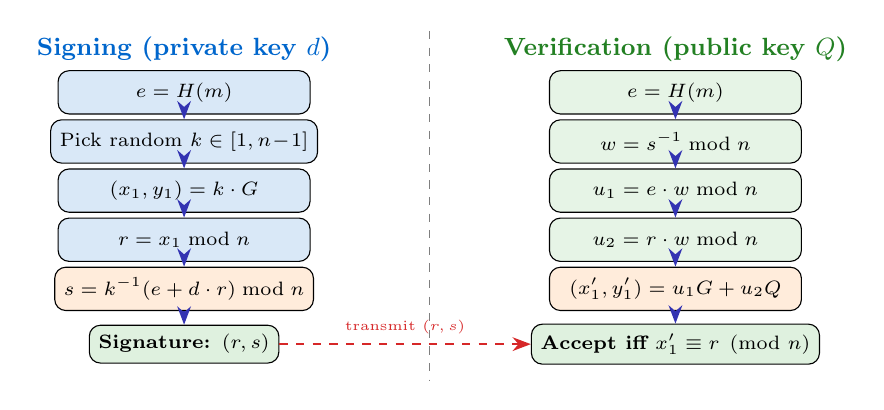
\begin{tikzpicture}[scale=0.78,
  box/.style={draw,rounded corners,minimum width=3.2cm,minimum height=0.55cm,font=\scriptsize,align=center},
  arr/.style={-{Stealth},thick,mlpurple}]
  % Signing column
  \node[font=\small\bfseries,mlblue] at (3,6.2) {Signing (private key $d$)};
  \node[box,fill=mlblue!15] (s1) at (3,5.5) {$e = H(m)$};
  \node[box,fill=mlblue!15] (s2) at (3,4.7) {Pick random $k \in [1,n\!-\!1]$};
  \node[box,fill=mlblue!15] (s3) at (3,3.9) {$(x_1, y_1) = k \cdot G$};
  \node[box,fill=mlblue!15] (s4) at (3,3.1) {$r = x_1 \bmod n$};
  \node[box,fill=mlorange!15] (s5) at (3,2.3) {$s = k^{-1}(e + d \cdot r) \bmod n$};
  \node[draw,rounded corners,fill=mlgreen!15,font=\scriptsize\bfseries] (sig) at (3,1.4) {Signature: $(r, s)$};
  \draw[arr] (s1)--(s2); \draw[arr] (s2)--(s3); \draw[arr] (s3)--(s4);
  \draw[arr] (s4)--(s5); \draw[arr] (s5)--(sig);
  % Verification column
  \node[font=\small\bfseries,mlgreen!80!black] at (11,6.2) {Verification (public key $Q$)};
  \node[box,fill=mlgreen!12] (v1) at (11,5.5) {$e = H(m)$};
  \node[box,fill=mlgreen!12] (v2) at (11,4.7) {$w = s^{-1} \bmod n$};
  \node[box,fill=mlgreen!12] (v3) at (11,3.9) {$u_1 = e \cdot w \bmod n$};
  \node[box,fill=mlgreen!12] (v4) at (11,3.1) {$u_2 = r \cdot w \bmod n$};
  \node[box,fill=mlorange!15] (v5) at (11,2.3) {$(x_1',y_1') = u_1 G + u_2 Q$};
  \node[draw,rounded corners,fill=mlgreen!15,font=\scriptsize\bfseries] (chk) at (11,1.4) {Accept iff $x_1' \equiv r \pmod{n}$};
  \draw[arr] (v1)--(v2); \draw[arr] (v2)--(v3); \draw[arr] (v3)--(v4);
  \draw[arr] (v4)--(v5); \draw[arr] (v5)--(chk);
  % Connecting arrow
  \draw[-{Stealth},thick,mlred,dashed] (sig.east) -- (chk.west) node[midway,above,font=\tiny,mlred]{transmit $(r,s)$};
  % Divider
  \draw[mlgray,dashed] (7,6.5) -- (7,0.8);
\end{tikzpicture}
\end{center}
\vspace{1mm}
\begin{alertblock}{Correctness}
\small $u_1 G + u_2 Q = u_1 G + u_2 dG = (u_1 + u_2 d)G = s^{-1}(e + dr)G = k G$, so $x$-coordinate matches $r$.
\end{alertblock}
\bottomnote{ECDSA (ANSI X9.62, 1998): the digital signature standard used in Bitcoin since block 0}
\end{frame}

%--- FRAME 26: Schnorr Signatures ---
\begin{frame}{Schnorr Signatures}
\begin{center}
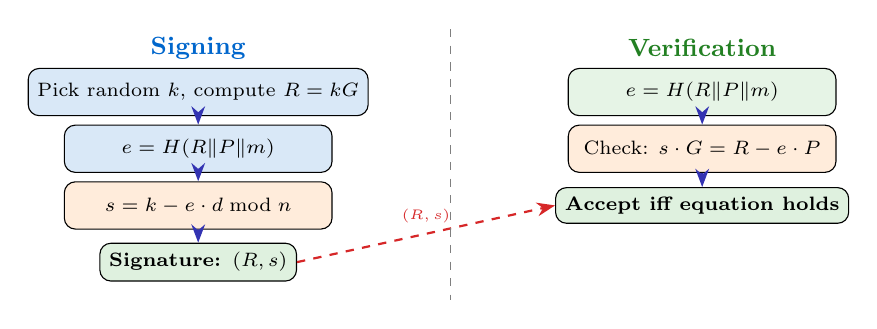
\begin{tikzpicture}[scale=0.8,
  box/.style={draw,rounded corners,minimum width=3.4cm,minimum height=0.6cm,font=\scriptsize,align=center},
  arr/.style={-{Stealth},thick,mlpurple}]
  % Signing
  \node[font=\small\bfseries,mlblue] at (3,5.2) {Signing};
  \node[box,fill=mlblue!15] (s1) at (3,4.5) {Pick random $k$, compute $R = kG$};
  \node[box,fill=mlblue!15] (s2) at (3,3.6) {$e = H(R \| P \| m)$};
  \node[box,fill=mlorange!15] (s3) at (3,2.7) {$s = k - e \cdot d \bmod n$};
  \node[draw,rounded corners,fill=mlgreen!15,font=\scriptsize\bfseries] (sig) at (3,1.8) {Signature: $(R, s)$};
  \draw[arr] (s1)--(s2); \draw[arr] (s2)--(s3); \draw[arr] (s3)--(sig);
  % Verification
  \node[font=\small\bfseries,mlgreen!80!black] at (11,5.2) {Verification};
  \node[box,fill=mlgreen!12] (v1) at (11,4.5) {$e = H(R \| P \| m)$};
  \node[box,fill=mlorange!15] (v2) at (11,3.6) {Check: $s \cdot G = R - e \cdot P$};
  \node[draw,rounded corners,fill=mlgreen!15,font=\scriptsize\bfseries] (chk) at (11,2.7) {Accept iff equation holds};
  \draw[arr] (v1)--(v2); \draw[arr] (v2)--(chk);
  % Arrow between
  \draw[-{Stealth},thick,mlred,dashed] (sig.east) -- (chk.west) node[midway,above,font=\tiny,mlred]{$(R,s)$};
  \draw[mlgray,dashed] (7,5.5) -- (7,1.2);
\end{tikzpicture}
\end{center}
\vspace{1mm}
\begin{columns}
\column{0.48\textwidth}
\begin{block}{Key Property: Linearity}
\small Schnorr signatures are \textbf{linear}: given signatures $(R_1,s_1)$ and $(R_2,s_2)$, one can combine them:
\[
  R = R_1 + R_2, \quad s = s_1 + s_2
\]
This enables native signature aggregation (MuSig).
\end{block}
\column{0.48\textwidth}
\begin{block}{Advantages over ECDSA}
\begin{itemize}\small
  \item \textbf{Provably secure} under random oracle model
  \item \textbf{Non-malleable}: unique encoding of $(R,s)$
  \item \textbf{Batch verification}: check multiple sigs faster
  \item \textbf{Simpler}: fewer operations than ECDSA
\end{itemize}
\end{block}
\begin{alertblock}{Bitcoin Taproot (BIP-340)}
\small Activated Nov 2021; uses Schnorr on secp256k1 (x-only public keys, 32 bytes).
\end{alertblock}
\end{columns}
\bottomnote{Schnorr (1989): patented until 2008 -- the reason Bitcoin initially used ECDSA instead}
\end{frame}

%--- FRAME 27: Signature Aggregation (MuSig) ---
\begin{frame}{Signature Aggregation: MuSig Protocol}
\begin{center}
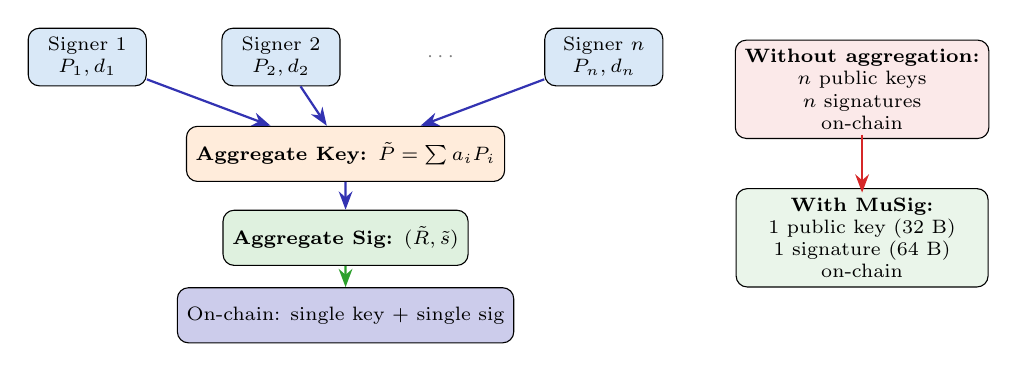
\begin{tikzpicture}[scale=0.82,
  signer/.style={draw,rounded corners,fill=mlblue!15,minimum width=1.5cm,minimum height=0.7cm,font=\scriptsize,align=center},
  agg/.style={draw,rounded corners,fill=mlgreen!15,minimum width=2.2cm,minimum height=0.7cm,font=\scriptsize\bfseries,align=center}]
  % Signers
  \node[signer] (p1) at (0,4) {Signer 1\\$P_1, d_1$};
  \node[signer] (p2) at (3,4) {Signer 2\\$P_2, d_2$};
  \node[font=\scriptsize,mlgray] at (5.5,4) {$\cdots$};
  \node[signer] (pn) at (8,4) {Signer $n$\\$P_n, d_n$};
  % Aggregate key
  \node[agg,fill=mlorange!15] (ak) at (4,2.5) {Aggregate Key: $\tilde{P} = \sum a_i P_i$};
  \draw[-{Stealth},mlpurple,thick] (p1) -- (ak);
  \draw[-{Stealth},mlpurple,thick] (p2) -- (ak);
  \draw[-{Stealth},mlpurple,thick] (pn) -- (ak);
  % Aggregate signature
  \node[agg] (as) at (4,1.2) {Aggregate Sig: $(\tilde{R}, \tilde{s})$};
  \draw[-{Stealth},mlpurple,thick] (ak) -- (as);
  % On-chain
  \node[draw,rounded corners,fill=mllavender3,minimum width=3cm,minimum height=0.7cm,font=\scriptsize] (chain) at (4,0) {On-chain: single key + single sig};
  \draw[-{Stealth},mlgreen,thick] (as) -- (chain);
  % Comparison
  \node[draw,rounded corners,fill=mlred!10,font=\scriptsize,align=center,minimum width=3.2cm] at (12,3.5) {\textbf{Without aggregation:}\\$n$ public keys\\$n$ signatures\\on-chain};
  \node[draw,rounded corners,fill=mlgreen!10,font=\scriptsize,align=center,minimum width=3.2cm] at (12,1.2) {\textbf{With MuSig:}\\1 public key (32~B)\\1 signature (64~B)\\on-chain};
  \draw[-{Stealth},thick,mlred] (12,2.8) -- (12,1.9);
\end{tikzpicture}
\end{center}
\vspace{2mm}
\begin{columns}
\column{0.48\textwidth}
\begin{block}{MuSig2 Protocol (3 rounds $\to$ 2 rounds)}
\begin{enumerate}\scriptsize
  \item Key aggregation: $a_i = H(L \| P_i)$, $\tilde{P} = \sum a_i P_i$
  \item Nonce exchange: each signer sends $R_i$; $\tilde{R} = \sum R_i$
  \item Partial sigs: $s_i = k_i + e \cdot a_i \cdot d_i$; aggregate $\tilde{s} = \sum s_i$
\end{enumerate}
\end{block}
\column{0.48\textwidth}
\begin{block}{Space Savings}
\begin{itemize}\small
  \item 100-of-100 multisig: from 6400~B to 96~B
  \item Indistinguishable from single-signer tx
  \item Improved fungibility and privacy
\end{itemize}
\end{block}
\end{columns}
\bottomnote{MuSig2 (2020): interactive 2-round protocol enabling key aggregation with provable security}
\end{frame}

%--- FRAME 28: Multi-Sig Schemes ---
\begin{frame}{Multi-Signature Schemes: $t$-of-$n$}
\begin{center}
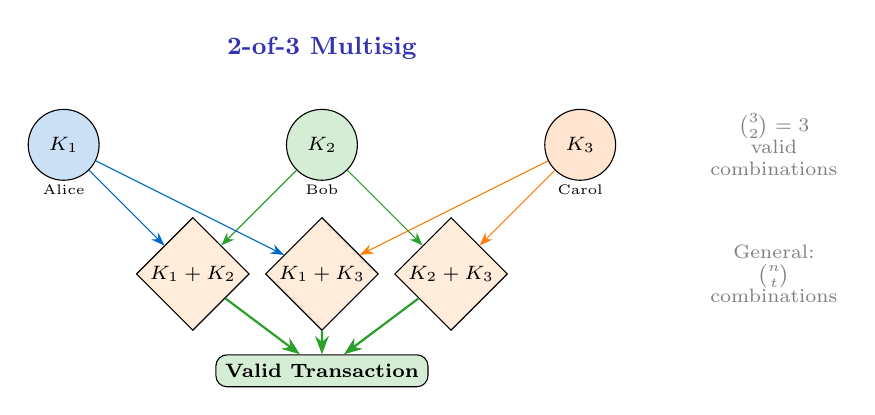
\begin{tikzpicture}[scale=0.82,
  key/.style={draw,circle,minimum size=0.9cm,font=\scriptsize\bfseries},
  decision/.style={draw,diamond,fill=mlorange!15,minimum width=1.2cm,minimum height=0.9cm,font=\scriptsize,align=center,inner sep=1pt}]
  % 2-of-3 example
  \node[font=\small\bfseries,mlpurple] at (4,5.5) {2-of-3 Multisig};
  \node[key,fill=mlblue!20] (k1) at (0,4) {$K_1$};
  \node[key,fill=mlgreen!20] (k2) at (4,4) {$K_2$};
  \node[key,fill=mlorange!20] (k3) at (8,4) {$K_3$};
  \node[font=\tiny] at (0,3.3) {Alice};
  \node[font=\tiny] at (4,3.3) {Bob};
  \node[font=\tiny] at (8,3.3) {Carol};
  % Valid combos
  \node[decision] (d1) at (2,2) {$K_1+K_2$};
  \node[decision] (d2) at (4,2) {$K_1+K_3$};
  \node[decision] (d3) at (6,2) {$K_2+K_3$};
  \draw[-{Stealth},mlblue] (k1) -- (d1);
  \draw[-{Stealth},mlgreen] (k2) -- (d1);
  \draw[-{Stealth},mlblue] (k1) -- (d2);
  \draw[-{Stealth},mlorange] (k3) -- (d2);
  \draw[-{Stealth},mlgreen] (k2) -- (d3);
  \draw[-{Stealth},mlorange] (k3) -- (d3);
  % All lead to valid
  \node[draw,rounded corners,fill=mlgreen!20,font=\scriptsize\bfseries] (valid) at (4,0.5) {Valid Transaction};
  \draw[-{Stealth},mlgreen,thick] (d1) -- (valid);
  \draw[-{Stealth},mlgreen,thick] (d2) -- (valid);
  \draw[-{Stealth},mlgreen,thick] (d3) -- (valid);
  % Count
  \node[font=\scriptsize,mlgray,align=center] at (11,4) {$\binom{3}{2} = 3$\\valid\\combinations};
  \node[font=\scriptsize,mlgray,align=center] at (11,2) {General:\\$\binom{n}{t}$\\combinations};
\end{tikzpicture}
\end{center}
\vspace{1mm}
\begin{columns}
\column{0.48\textwidth}
\begin{block}{Implementation Approaches}
\begin{itemize}\small
  \item \textbf{Script-based} (Bitcoin P2SH): explicit $t$-of-$n$ in script
  \item \textbf{Schnorr/MuSig}: aggregated on-chain (Taproot)
  \item \textbf{Shamir + MPC}: threshold signatures off-chain
\end{itemize}
\end{block}
\column{0.48\textwidth}
\begin{block}{Common Configurations}
\scriptsize
\begin{tabular}{ll}
\toprule
\textbf{Setup} & \textbf{Use Case} \\
\midrule
2-of-3 & Personal wallet + backup + partner \\
3-of-5 & Corporate treasury \\
6-of-9 & DAO governance \\
$n$-of-$n$ & Unanimous consent (Lightning) \\
\bottomrule
\end{tabular}
\end{block}
\end{columns}
\bottomnote{Multi-sig eliminates single points of failure: no single key compromise can drain funds}
\end{frame}

%--- FRAME 29: Nonce Reuse Vulnerability ---
\begin{frame}{Nonce Reuse Vulnerability}
\begin{center}
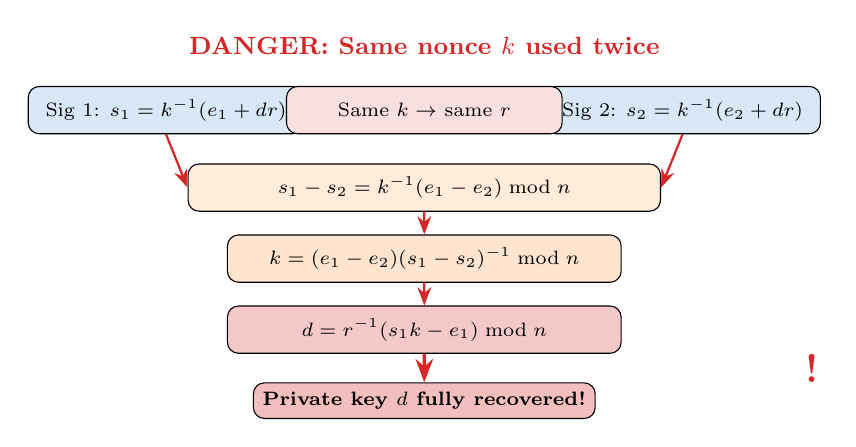
\begin{tikzpicture}[scale=0.82,
  box/.style={draw,rounded corners,minimum width=3.5cm,minimum height=0.6cm,font=\scriptsize,align=center}]
  % Two signatures with same k
  \node[font=\small\bfseries,mlred] at (4,6) {DANGER: Same nonce $k$ used twice};
  \node[box,fill=mlblue!15] (sig1) at (0,5) {Sig 1: $s_1 = k^{-1}(e_1 + dr)$};
  \node[box,fill=mlblue!15] (sig2) at (8,5) {Sig 2: $s_2 = k^{-1}(e_2 + dr)$};
  \node[box,fill=mlred!15] (same) at (4,5) {Same $k \to$ same $r$};
  % Attack step
  \node[box,fill=mlorange!15,minimum width=6cm] (diff) at (4,3.8) {$s_1 - s_2 = k^{-1}(e_1 - e_2) \bmod n$};
  \draw[-{Stealth},mlred,thick] (sig1.south) -- (diff.west);
  \draw[-{Stealth},mlred,thick] (sig2.south) -- (diff.east);
  % Extract k
  \node[box,fill=mlorange!20,minimum width=5cm] (getk) at (4,2.7) {$k = (e_1 - e_2)(s_1 - s_2)^{-1} \bmod n$};
  \draw[-{Stealth},mlred,thick] (diff) -- (getk);
  % Extract d
  \node[box,fill=mlred!25,minimum width=5cm] (getd) at (4,1.6) {$d = r^{-1}(s_1 k - e_1) \bmod n$};
  \draw[-{Stealth},mlred,thick] (getk) -- (getd);
  % Result
  \node[draw,rounded corners,fill=mlred!30,font=\scriptsize\bfseries,minimum width=4cm] (priv) at (4,0.5) {Private key $d$ fully recovered!};
  \draw[-{Stealth},mlred,very thick] (getd) -- (priv);
  % Warning icon
  \node[font=\Large,mlred] at (10,1) {\textbf{!}};
\end{tikzpicture}
\end{center}
\vspace{1mm}
\begin{columns}
\column{0.48\textwidth}
\begin{block}{Real-World Incidents}
\begin{itemize}\small
  \item \textbf{Sony PS3 (2010)}: ECDSA with constant $k$; entire private key extracted; enabled homebrew
  \item \textbf{Android Bitcoin wallets (2013)}: faulty SecureRandom reused $k$ values
  \item \textbf{Blockchain.info (2014)}: weak RNG led to nonce collisions
\end{itemize}
\end{block}
\column{0.48\textwidth}
\begin{block}{Defenses}
\begin{itemize}\small
  \item \textbf{RFC 6979}: deterministic $k = \text{HMAC}(d, H(m))$
  \item \textbf{Ed25519}: nonce derived from private key hash (by design)
  \item \textbf{Schnorr BIP-340}: auxiliary randomness mixed in
  \item Never use raw \texttt{random()} for nonce generation
\end{itemize}
\end{block}
\end{columns}
\bottomnote{A single nonce reuse leaks the entire private key -- the most dangerous implementation error in ECDSA}
\end{frame}

%--- FRAME 30: Batch Verification ---
\begin{frame}{Batch Verification Performance}
\begin{center}
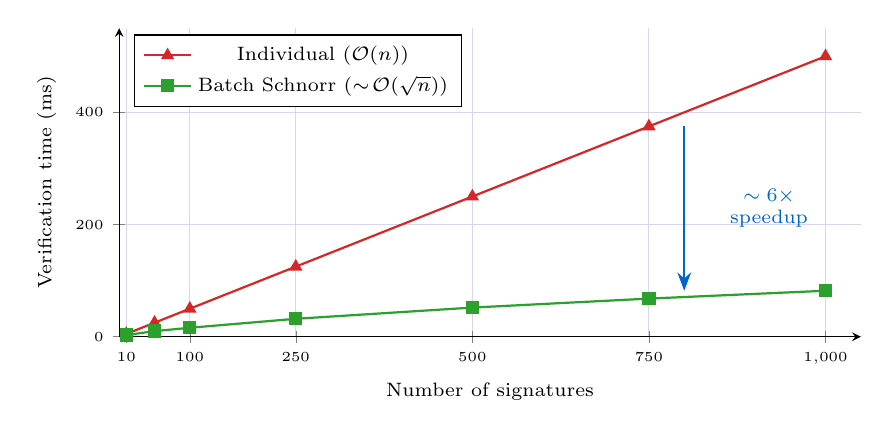
\begin{tikzpicture}
\begin{axis}[
  width=11cm, height=5.5cm,
  xlabel={\scriptsize Number of signatures},
  ylabel={\scriptsize Verification time (ms)},
  xmin=0, xmax=1050,
  ymin=0, ymax=550,
  grid=major,
  grid style={mllavender4},
  axis lines=left,
  xlabel style={font=\scriptsize},
  ylabel style={font=\scriptsize},
  tick label style={font=\tiny},
  legend style={font=\scriptsize,at={(0.02,0.98)},anchor=north west},
  xtick={10,100,250,500,750,1000},
]
% Individual verification: linear
\addplot[mlred,thick,mark=triangle*,mark size=2pt] coordinates {
  (10,5) (50,25) (100,50) (250,125) (500,250) (750,375) (1000,500)
};
\addlegendentry{Individual ($\mathcal{O}(n)$)}
% Batch verification: sublinear
\addplot[mlgreen,thick,mark=square*,mark size=2pt] coordinates {
  (10,3) (50,10) (100,16) (250,32) (500,52) (750,68) (1000,82)
};
\addlegendentry{Batch Schnorr ($\sim\!\mathcal{O}(\sqrt{n})$)}
% Speedup annotation
\draw[-{Stealth},mlblue,thick] (axis cs:800,375) -- (axis cs:800,82);
\node[font=\scriptsize,mlblue,align=center] at (axis cs:920,230) {$\sim 6\times$\\speedup};
\end{axis}
\end{tikzpicture}
\end{center}
\vspace{1mm}
\begin{columns}
\column{0.48\textwidth}
\begin{block}{How Batch Verification Works}
\small Instead of $n$ individual checks $s_i G = R_i + e_i P_i$, compute one multi-scalar multiplication:
\[
  \left(\sum z_i s_i\right) G = \sum z_i R_i + \sum z_i e_i P_i
\]
where $z_i$ are random weights (for soundness).
\end{block}
\column{0.48\textwidth}
\begin{block}{Blockchain Impact}
\begin{itemize}\small
  \item \textbf{Block validation}: verify all txs in a block at once
  \item \textbf{Node sync}: significantly faster initial block download
  \item \textbf{Schnorr advantage}: ECDSA does not support batch verification
  \item Saves $\sim 50\%$ CPU during peak load
\end{itemize}
\end{block}
\end{columns}
\bottomnote{Batch verification is a key advantage of Schnorr over ECDSA -- enabled in Bitcoin via Taproot (BIP-340)}
\end{frame}

%--- FRAME 31: Signature Schemes Comparison ---
\begin{frame}{Signature Schemes Comparison}
\begin{center}
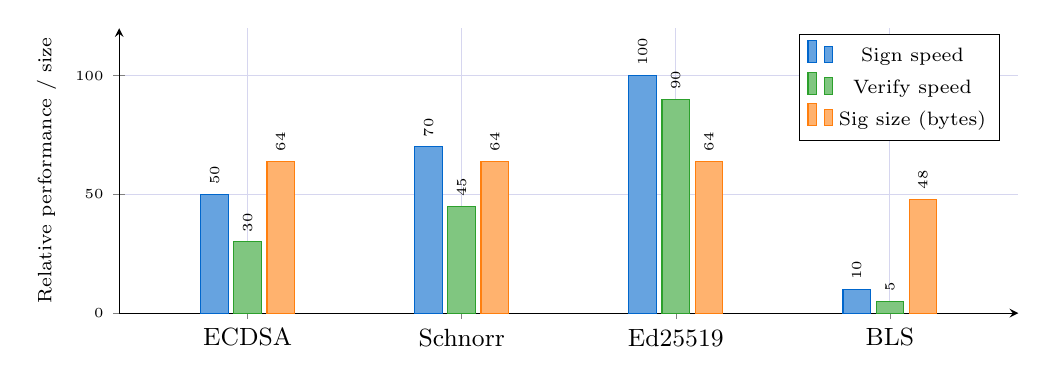
\begin{tikzpicture}
\begin{axis}[
  ybar,
  width=13cm, height=5.2cm,
  ylabel={\scriptsize Relative performance / size},
  symbolic x coords={ECDSA,Schnorr,Ed25519,BLS},
  xtick=data,
  x tick label style={font=\small},
  y tick label style={font=\tiny},
  ymin=0, ymax=120,
  bar width=0.35cm,
  axis lines=left,
  grid=major,
  grid style={mllavender4},
  ylabel style={font=\scriptsize},
  legend style={font=\scriptsize,at={(0.98,0.98)},anchor=north east},
  nodes near coords,
  nodes near coords style={font=\tiny,rotate=90,anchor=west},
  enlarge x limits=0.2,
]
\addplot[fill=mlblue!60,draw=mlblue] coordinates {(ECDSA,50) (Schnorr,70) (Ed25519,100) (BLS,10)};
\addlegendentry{Sign speed}
\addplot[fill=mlgreen!60,draw=mlgreen] coordinates {(ECDSA,30) (Schnorr,45) (Ed25519,90) (BLS,5)};
\addlegendentry{Verify speed}
\addplot[fill=mlorange!60,draw=mlorange] coordinates {(ECDSA,64) (Schnorr,64) (Ed25519,64) (BLS,48)};
\addlegendentry{Sig size (bytes)}
\end{axis}
\end{tikzpicture}
\end{center}
\vspace{1mm}
\begin{columns}
\column{0.48\textwidth}
\begin{block}{Feature Matrix}
\scriptsize
\begin{tabular}{lcccc}
\toprule
& \textbf{ECDSA} & \textbf{Schnorr} & \textbf{Ed25519} & \textbf{BLS} \\
\midrule
Batch verify & \textcolor{mlred}{\texttimes} & \checkmark & \checkmark & \checkmark \\
Aggregation & \textcolor{mlred}{\texttimes} & \checkmark & \textcolor{mlred}{\texttimes} & \checkmark \\
Det.\ nonce & RFC6979 & BIP-340 & Native & -- \\
Pairing-free & \checkmark & \checkmark & \checkmark & \textcolor{mlred}{\texttimes} \\
\bottomrule
\end{tabular}
\end{block}
\column{0.48\textwidth}
\begin{block}{When to Use Which}
\begin{itemize}\small
  \item \textbf{ECDSA}: legacy compatibility (Bitcoin, Ethereum)
  \item \textbf{Schnorr}: aggregation, Taproot multisig
  \item \textbf{Ed25519}: new chains (Solana, Cardano)
  \item \textbf{BLS}: consensus sigs (Ethereum 2.0 validators)
\end{itemize}
\end{block}
\end{columns}
\bottomnote{BLS signatures enable $n$ validator signatures to aggregate into a single 48-byte proof -- essential for PoS scalability}
\end{frame}

\section{Key Management \& Wallets}

%--- FRAME 32: BIP-39 Mnemonic Seeds ---
\begin{frame}{BIP-39: Mnemonic Seed Phrases}
\begin{center}
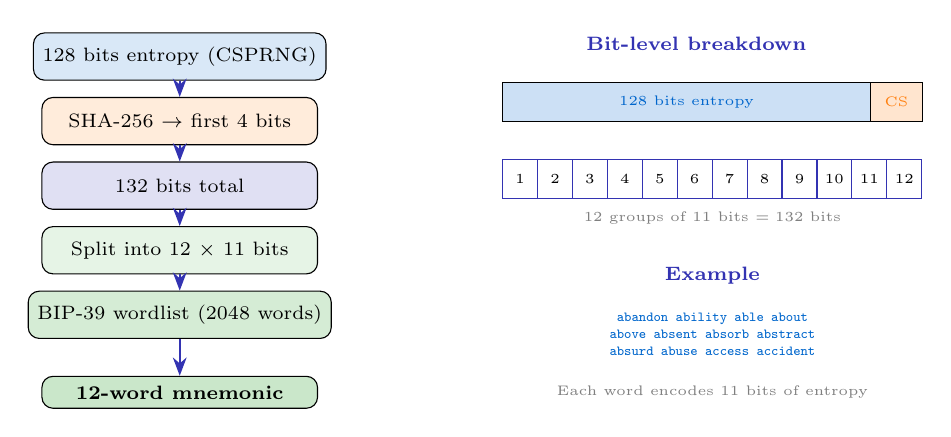
\begin{tikzpicture}[scale=0.82,
  box/.style={draw,rounded corners,minimum width=2.2cm,minimum height=0.6cm,font=\scriptsize,align=center},
  arr/.style={-{Stealth},thick,mlpurple}]
  % Entropy
  \node[box,fill=mlblue!15,minimum width=3.5cm] (ent) at (0,4) {128 bits entropy (CSPRNG)};
  % Checksum
  \node[box,fill=mlorange!15,minimum width=3.5cm] (cs) at (0,3) {SHA-256 $\to$ first 4 bits};
  \draw[arr] (ent) -- (cs);
  % Combined
  \node[box,fill=mlpurple!15,minimum width=3.5cm] (comb) at (0,2) {132 bits total};
  \draw[arr] (cs) -- (comb);
  % Split
  \node[box,fill=mlgreen!12,minimum width=3.5cm] (split) at (0,1) {Split into 12 $\times$ 11 bits};
  \draw[arr] (comb) -- (split);
  % Word lookup
  \node[box,fill=mlgreen!20,minimum width=3.5cm] (words) at (0,0) {BIP-39 wordlist (2048 words)};
  \draw[arr] (split) -- (words);
  % Result
  \node[draw,rounded corners,fill=mlgreen!25,font=\scriptsize\bfseries,minimum width=3.5cm] (mn) at (0,-1.2) {12-word mnemonic};
  \draw[arr] (words) -- (mn);
  % Bit-level breakdown
  \node[font=\scriptsize\bfseries,mlpurple] at (8,4.2) {Bit-level breakdown};
  \draw[mlgray] (5,3.6) rectangle (11.5,3.0);
  \draw[fill=mlblue!20] (5,3.6) rectangle (10.7,3.0);
  \node[font=\tiny,mlblue] at (7.85,3.3) {128 bits entropy};
  \draw[fill=mlorange!20] (10.7,3.6) rectangle (11.5,3.0);
  \node[font=\tiny,mlorange] at (11.1,3.3) {CS};
  % 11-bit groups
  \foreach \i in {0,...,11}{
    \pgfmathsetmacro{\xl}{5 + \i*0.541}
    \pgfmathsetmacro{\xr}{5 + (\i+1)*0.541}
    \draw[mlpurple] (\xl,2.4) rectangle (\xr,1.8);
    \node[font=\tiny] at ({(\xl+\xr)/2},2.1) {\pgfmathparse{int(\i+1)}\pgfmathresult};
  }
  \node[font=\tiny,mlgray] at (8.25,1.5) {12 groups of 11 bits $= 132$ bits};
  % Example
  \node[font=\scriptsize\bfseries,mlpurple] at (8.25,0.6) {Example};
  \node[font=\tiny,align=center,mlblue] at (8.25,-0.3) {\texttt{abandon ability able about}\\
  \texttt{above absent absorb abstract}\\
  \texttt{absurd abuse access accident}};
  \node[font=\tiny,mlgray] at (8.25,-1.2) {Each word encodes 11 bits of entropy};
\end{tikzpicture}
\end{center}
\vspace{1mm}
\begin{alertblock}{Entropy $\to$ Mnemonic $\to$ Seed}
\small Mnemonic + optional passphrase $\xrightarrow{\text{PBKDF2 (2048 rounds)}}$ 512-bit seed $\to$ master key for HD wallet (BIP-32).
\end{alertblock}
\bottomnote{BIP-39 supports 12, 15, 18, 21, or 24 words (128--256 bits entropy); human-readable backup of all keys}
\end{frame}

%--- FRAME 33: BIP-32 HD Wallets ---
\begin{frame}{BIP-32: Hierarchical Deterministic Wallets}
\begin{center}
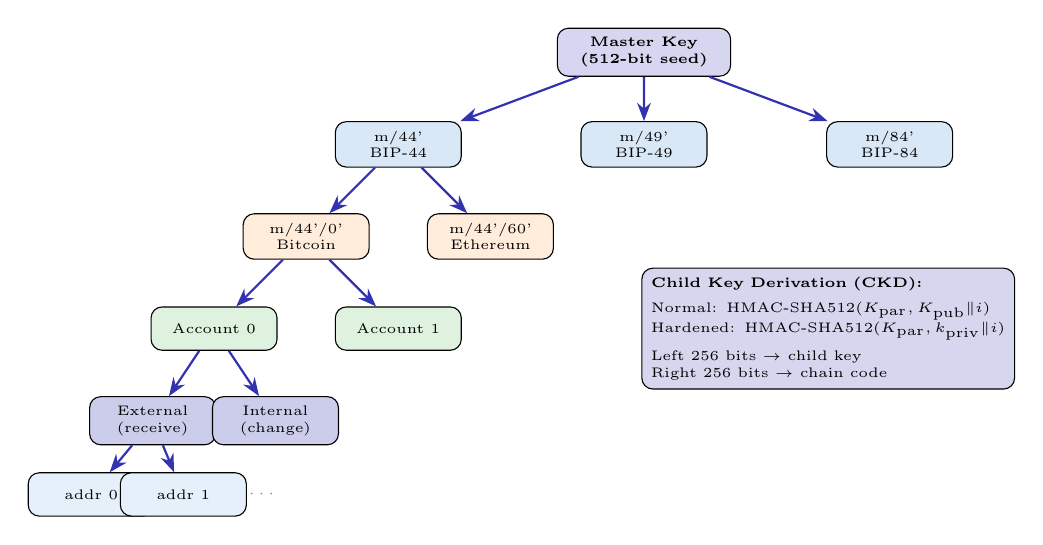
\begin{tikzpicture}[scale=0.78,
  node/.style={draw,rounded corners,minimum width=1.6cm,minimum height=0.55cm,font=\tiny,align=center},
  edge/.style={-{Stealth},thick,mlpurple}]
  % Master
  \node[node,fill=mlpurple!20,minimum width=2.2cm,font=\tiny\bfseries] (m) at (7,6) {Master Key\\(512-bit seed)};
  % Purpose level
  \node[node,fill=mlblue!15] (p44) at (3,4.5) {m/44'\\BIP-44};
  \node[node,fill=mlblue!15] (p49) at (7,4.5) {m/49'\\BIP-49};
  \node[node,fill=mlblue!15] (p84) at (11,4.5) {m/84'\\BIP-84};
  \draw[edge] (m) -- (p44); \draw[edge] (m) -- (p49); \draw[edge] (m) -- (p84);
  % Coin type
  \node[node,fill=mlorange!15] (btc) at (1.5,3) {m/44'/0'\\Bitcoin};
  \node[node,fill=mlorange!15] (eth) at (4.5,3) {m/44'/60'\\Ethereum};
  \draw[edge] (p44) -- (btc); \draw[edge] (p44) -- (eth);
  % Account
  \node[node,fill=mlgreen!15] (a0) at (0,1.5) {Account 0};
  \node[node,fill=mlgreen!15] (a1) at (3,1.5) {Account 1};
  \draw[edge] (btc) -- (a0); \draw[edge] (btc) -- (a1);
  % Change
  \node[node,fill=mllavender3] (ext) at (-1,0) {External\\(receive)};
  \node[node,fill=mllavender3] (int) at (1,0) {Internal\\(change)};
  \draw[edge] (a0) -- (ext); \draw[edge] (a0) -- (int);
  % Addresses
  \node[node,fill=mlblue!10,font=\tiny] (ad0) at (-2,-1.2) {addr 0};
  \node[node,fill=mlblue!10,font=\tiny] (ad1) at (-0.5,-1.2) {addr 1};
  \node[font=\tiny,mlgray] at (0.8,-1.2) {$\cdots$};
  \draw[edge] (ext) -- (ad0); \draw[edge] (ext) -- (ad1);
  % CKD box
  \node[draw,rounded corners,fill=mllavender4,font=\tiny,align=left,text width=4.5cm] at (10,1.5) {
    \textbf{Child Key Derivation (CKD):}\\[1mm]
    Normal: $\text{HMAC-SHA512}(K_{\text{par}}, K_{\text{pub}} \| i)$\\
    Hardened: $\text{HMAC-SHA512}(K_{\text{par}}, k_{\text{priv}} \| i)$\\[1mm]
    Left 256 bits $\to$ child key\\
    Right 256 bits $\to$ chain code
  };
\end{tikzpicture}
\end{center}
\vspace{1mm}
\begin{columns}
\column{0.48\textwidth}
\begin{block}{Key Properties}
\begin{itemize}\small
  \item Single seed $\to$ unlimited keys
  \item Deterministic: same seed $=$ same keys
  \item Tree structure with purpose/coin/account levels
\end{itemize}
\end{block}
\column{0.48\textwidth}
\begin{block}{Normal vs.\ Hardened Derivation}
\begin{itemize}\small
  \item \textbf{Normal} ($i < 2^{31}$): xpub can derive child public keys
  \item \textbf{Hardened} ($i \geq 2^{31}$, marked $'$): requires parent private key
  \item Hardened prevents xpub+child leak $\to$ master leak
\end{itemize}
\end{block}
\end{columns}
\bottomnote{BIP-32 (2012): one backup (seed phrase) secures all current and future keys across all coins}
\end{frame}

%--- FRAME 34: BIP-44 Multi-Account Hierarchy ---
\begin{frame}{BIP-44: Multi-Account HD Derivation Paths}
\begin{block}{Standard Derivation Path}
\[
  \texttt{m / purpose' / coin\_type' / account' / change / address\_index}
\]
\end{block}
\vspace{2mm}
\begin{center}
\small
\begin{tabular}{llll}
\toprule
\textbf{Level} & \textbf{Field} & \textbf{Values} & \textbf{Description} \\
\midrule
1 & Purpose & $44'$ (BIP-44), $49'$ (SegWit), $84'$ (native SegWit) & Wallet standard \\
2 & Coin type & $0'$ = BTC, $60'$ = ETH, $501'$ = SOL & SLIP-44 registry \\
3 & Account & $0', 1', 2', \ldots$ & User accounts \\
4 & Change & $0$ = external (receive), $1$ = internal (change) & Address role \\
5 & Index & $0, 1, 2, \ldots$ & Sequential addresses \\
\bottomrule
\end{tabular}
\end{center}
\vspace{3mm}
\begin{columns}
\column{0.48\textwidth}
\begin{block}{Example Paths}
\scriptsize
\begin{tabular}{ll}
\toprule
\textbf{Path} & \textbf{Meaning} \\
\midrule
\texttt{m/44'/0'/0'/0/0} & 1st BTC receive address \\
\texttt{m/44'/0'/0'/1/0} & 1st BTC change address \\
\texttt{m/44'/0'/1'/0/0} & 2nd BTC account, 1st addr \\
\texttt{m/44'/60'/0'/0/0} & 1st ETH address \\
\texttt{m/84'/0'/0'/0/0} & 1st native SegWit BTC addr \\
\bottomrule
\end{tabular}
\end{block}
\column{0.48\textwidth}
\begin{block}{Why Standardized Paths Matter}
\begin{itemize}\small
  \item \textbf{Interoperability}: import seed in any BIP-44 wallet
  \item \textbf{Recovery}: deterministic path $=$ predictable keys
  \item \textbf{Privacy}: new address per transaction (gap limit 20)
  \item \textbf{Organization}: separate accounts for different purposes
\end{itemize}
\end{block}
\end{columns}
\bottomnote{BIP-44 enables wallet portability: the same 12/24 words work across Ledger, Trezor, MetaMask, and Electrum}
\end{frame}

%--- FRAME 35: Key Derivation Security Analysis ---
\begin{frame}{Key Derivation Security Analysis}
\begin{center}
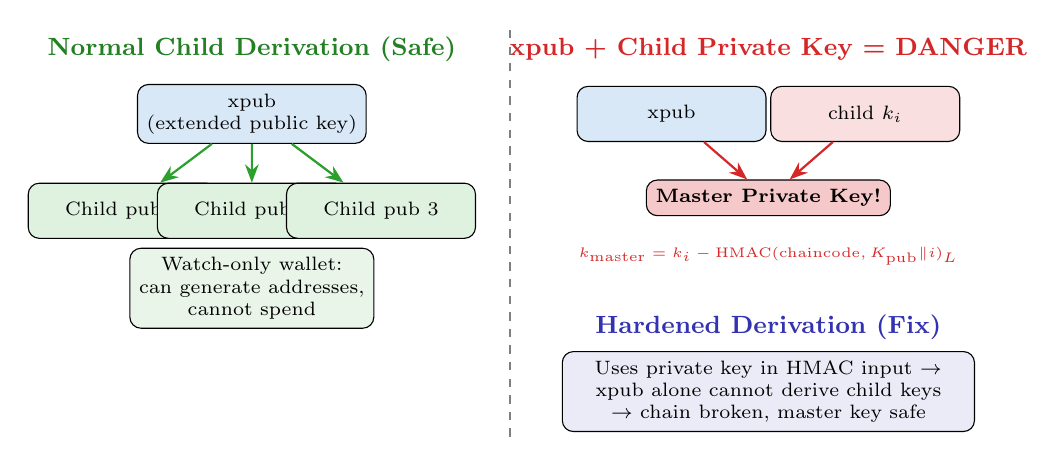
\begin{tikzpicture}[scale=0.82,
  box/.style={draw,rounded corners,minimum width=2.4cm,minimum height=0.7cm,font=\scriptsize,align=center},
  arr/.style={-{Stealth},thick}]
  % Safe side: Normal derivation
  \node[font=\small\bfseries,mlgreen!80!black] at (3,5.5) {Normal Child Derivation (Safe)};
  \node[box,fill=mlblue!15] (xpub) at (3,4.5) {xpub\\(extended public key)};
  \node[box,fill=mlgreen!15] (cpub1) at (1,3) {Child pub 1};
  \node[box,fill=mlgreen!15] (cpub2) at (3,3) {Child pub 2};
  \node[box,fill=mlgreen!15] (cpub3) at (5,3) {Child pub 3};
  \draw[arr,mlgreen] (xpub) -- (cpub1);
  \draw[arr,mlgreen] (xpub) -- (cpub2);
  \draw[arr,mlgreen] (xpub) -- (cpub3);
  \node[draw,rounded corners,fill=mlgreen!10,font=\scriptsize,align=center] at (3,1.8) {Watch-only wallet:\\can generate addresses,\\cannot spend};
  % Danger side
  \node[font=\small\bfseries,mlred] at (11,5.5) {xpub + Child Private Key = DANGER};
  \node[box,fill=mlblue!15] (xpub2) at (9.5,4.5) {xpub};
  \node[box,fill=mlred!15] (cpriv) at (12.5,4.5) {child $k_i$};
  \node[draw,rounded corners,fill=mlred!25,font=\scriptsize\bfseries,minimum width=3cm] (master) at (11,3.2) {Master Private Key!};
  \draw[arr,mlred] (xpub2) -- (master);
  \draw[arr,mlred] (cpriv) -- (master);
  \node[font=\tiny,mlred,align=center] at (11,2.3) {$k_{\text{master}} = k_i - \text{HMAC}(\text{chaincode}, K_{\text{pub}} \| i)_L$};
  % Hardened fix
  \node[font=\small\bfseries,mlpurple] at (11,1.2) {Hardened Derivation (Fix)};
  \node[draw,rounded corners,fill=mlpurple!10,font=\scriptsize,align=center,text width=5cm] at (11,0.2) {Uses private key in HMAC input $\to$\\xpub alone cannot derive child keys\\$\to$ chain broken, master key safe};
  % Divider
  \draw[mlgray,dashed,thick] (7,5.8) -- (7,-0.5);
\end{tikzpicture}
\end{center}
\vspace{1mm}
\begin{alertblock}{Critical Rule}
\small \textbf{Never share xpub if any child private key might be exposed.} Use hardened derivation (indicated by $'$) for account-level keys. Normal derivation is safe only below the hardened boundary.
\end{alertblock}
\bottomnote{This is why BIP-44 uses hardened derivation for purpose, coin type, and account levels}
\end{frame}

%--- FRAME 36: Hardware Wallet Architecture ---
\begin{frame}{Hardware Wallet Architecture}
\begin{center}
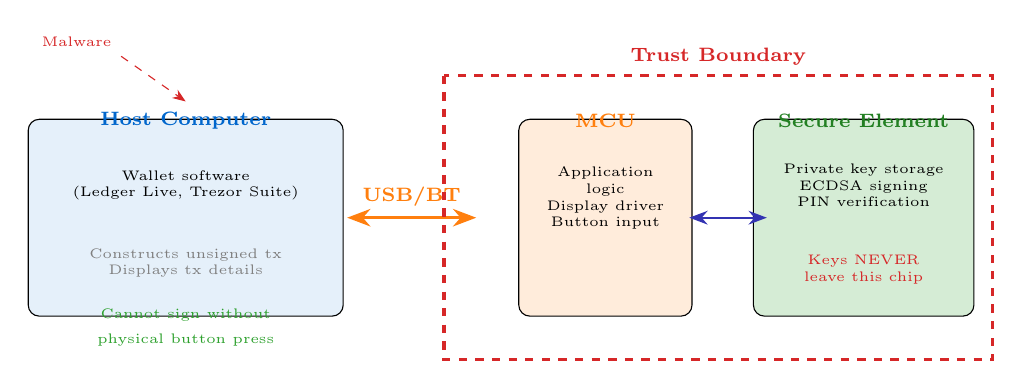
\begin{tikzpicture}[scale=0.82,
  comp/.style={draw,rounded corners,minimum width=2.2cm,minimum height=1.0cm,font=\scriptsize,align=center}]
  % Host computer
  \node[comp,fill=mlblue!10,minimum width=4cm,minimum height=2.5cm] (host) at (0,2) {};
  \node[font=\scriptsize\bfseries,mlblue] at (0,3.5) {Host Computer};
  \node[font=\tiny,align=center] at (0,2.5) {Wallet software\\(Ledger Live, Trezor Suite)};
  \node[font=\tiny,align=center,mlgray] at (0,1.3) {Constructs unsigned tx\\Displays tx details};
  % USB connection
  \draw[{Stealth}-{Stealth},very thick,mlorange] (2.5,2) -- (4.5,2) node[midway,above,font=\scriptsize\bfseries]{USB/BT};
  % MCU
  \node[comp,fill=mlorange!15,minimum width=2.2cm,minimum height=2.5cm] (mcu) at (6.5,2) {};
  \node[font=\scriptsize\bfseries,mlorange] at (6.5,3.5) {MCU};
  \node[font=\tiny,align=center] at (6.5,2.3) {Application\\logic\\Display driver\\Button input};
  % Secure Element
  \node[comp,fill=mlgreen!20,minimum width=2.8cm,minimum height=2.5cm] (se) at (10.5,2) {};
  \node[font=\scriptsize\bfseries,mlgreen!80!black] at (10.5,3.5) {Secure Element};
  \node[font=\tiny,align=center] at (10.5,2.5) {Private key storage\\ECDSA signing\\PIN verification};
  \node[font=\tiny,mlred,align=center] at (10.5,1.2) {Keys NEVER\\leave this chip};
  \draw[{Stealth}-{Stealth},thick,mlpurple] (7.8,2) -- (9,2);
  % Trust boundary
  \draw[mlred,very thick,dashed] (4.0,4.2) rectangle (12.5,-0.2);
  \node[font=\scriptsize\bfseries,mlred] at (8.25,4.5) {Trust Boundary};
  % Attack arrows
  \draw[-{Stealth},mlred,dashed] (-1,4.5) -- (0,3.8) node[above left,font=\tiny,mlred,pos=0]{Malware};
  \node[font=\tiny,mlgreen] at (0,0.5) {Cannot sign without};
  \node[font=\tiny,mlgreen] at (0,0.1) {physical button press};
\end{tikzpicture}
\end{center}
\vspace{2mm}
\begin{columns}
\column{0.48\textwidth}
\begin{block}{Security Model}
\begin{itemize}\small
  \item \textbf{Air gap}: keys generated and stored on-device
  \item \textbf{Physical confirmation}: button press required
  \item \textbf{Tamper resistance}: secure element detects physical attacks
  \item \textbf{Open source firmware}: verifiable signing logic
\end{itemize}
\end{block}
\column{0.48\textwidth}
\begin{block}{Threat Mitigation}
\scriptsize
\begin{tabular}{ll}
\toprule
\textbf{Threat} & \textbf{Defense} \\
\midrule
Malware on host & Keys never on host \\
Supply chain attack & Attestation + open firmware \\
Physical theft & PIN + passphrase \\
Firmware backdoor & Reproducible builds \\
Side-channel & Secure element hardening \\
\bottomrule
\end{tabular}
\end{block}
\end{columns}
\bottomnote{Hardware wallets (Ledger, Trezor, Coldcard) provide the strongest practical key security for individual users}
\end{frame}

%--- FRAME 37: Wallet Recovery & Inheritance ---
\begin{frame}{Wallet Recovery: Shamir's Secret Sharing}
\begin{center}
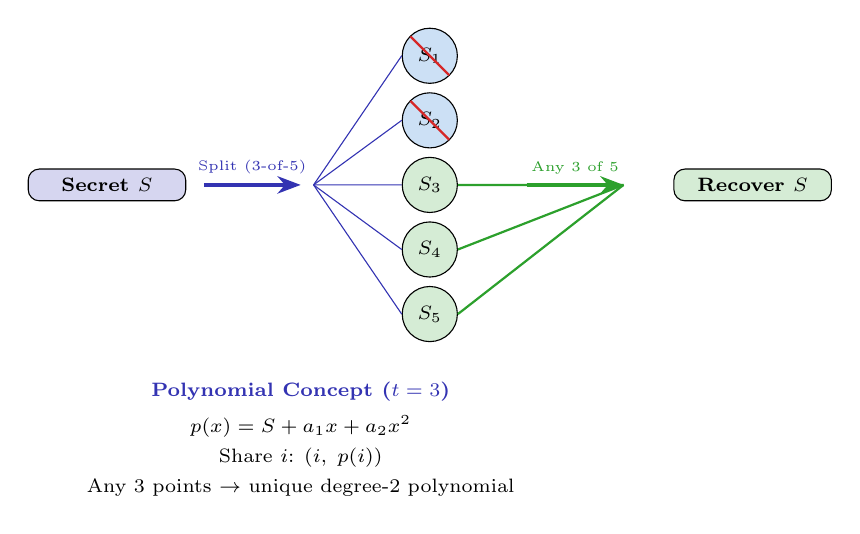
\begin{tikzpicture}[scale=0.82,
  share/.style={draw,circle,minimum size=0.7cm,font=\scriptsize\bfseries}]
  % Secret
  \node[draw,rounded corners,fill=mlpurple!20,minimum width=2cm,font=\scriptsize\bfseries] (secret) at (0,3) {Secret $S$};
  % Split arrow
  \draw[-{Stealth},mlpurple,very thick] (1.5,3) -- (3,3) node[midway,above,font=\tiny]{Split (3-of-5)};
  % 5 shares
  \node[share,fill=mlblue!20] (s1) at (5,5) {$S_1$};
  \node[share,fill=mlblue!20] (s2) at (5,4) {$S_2$};
  \node[share,fill=mlgreen!20] (s3) at (5,3) {$S_3$};
  \node[share,fill=mlgreen!20] (s4) at (5,2) {$S_4$};
  \node[share,fill=mlgreen!20] (s5) at (5,1) {$S_5$};
  \draw[mlpurple] (3.2,3) -- (s1.west);
  \draw[mlpurple] (3.2,3) -- (s2.west);
  \draw[mlpurple] (3.2,3) -- (s3.west);
  \draw[mlpurple] (3.2,3) -- (s4.west);
  \draw[mlpurple] (3.2,3) -- (s5.west);
  % Reconstruction
  \draw[-{Stealth},mlgreen,very thick] (6.5,3) -- (8,3) node[midway,above,font=\tiny]{Any 3 of 5};
  \node[draw,rounded corners,fill=mlgreen!20,minimum width=2cm,font=\scriptsize\bfseries] (rec) at (10,3) {Recover $S$};
  % Highlight 3 chosen shares
  \draw[mlgreen,thick] (s3.east) -- (8,3);
  \draw[mlgreen,thick] (s4.east) -- (8,3);
  \draw[mlgreen,thick] (s5.east) -- (8,3);
  % Crossed out (not needed)
  \draw[mlred,thick] (4.7,5.3) -- (5.3,4.7);
  \draw[mlred,thick] (4.7,4.3) -- (5.3,3.7);
  % Polynomial concept
  \node[font=\scriptsize\bfseries,mlpurple] at (3,-0.2) {Polynomial Concept ($t=3$)};
  \node[font=\scriptsize,align=center] at (3,-1.2) {$p(x) = S + a_1 x + a_2 x^2$\\[1mm]
    Share $i$: $(i,\; p(i))$\\[1mm]
    Any 3 points $\to$ unique degree-2 polynomial};
\end{tikzpicture}
\end{center}
\vspace{1mm}
\begin{columns}
\column{0.48\textwidth}
\begin{block}{Properties}
\begin{itemize}\small
  \item \textbf{Information-theoretic}: $t\!-\!1$ shares reveal \emph{zero} information
  \item \textbf{Flexible}: any $t$-of-$n$ threshold
  \item \textbf{SLIP-39}: standardized for wallets (differs from BIP-39)
\end{itemize}
\end{block}
\column{0.48\textwidth}
\begin{block}{Inheritance Planning}
\begin{itemize}\small
  \item 2-of-3: owner, spouse, lawyer
  \item 3-of-5: geographic distribution (safe deposit boxes)
  \item Time-locked: dead man's switch via smart contract
  \item Multi-generational: hierarchical share distribution
\end{itemize}
\end{block}
\end{columns}
\bottomnote{Shamir (1979): $t$-of-$n$ secret sharing is information-theoretically secure -- no computational assumptions needed}
\end{frame}

\section{Cryptographic Protocols}

%--- FRAME 38: Zero-Knowledge Proofs Concept ---
\begin{frame}{Zero-Knowledge Proofs: The Ali Baba Cave}
\begin{center}
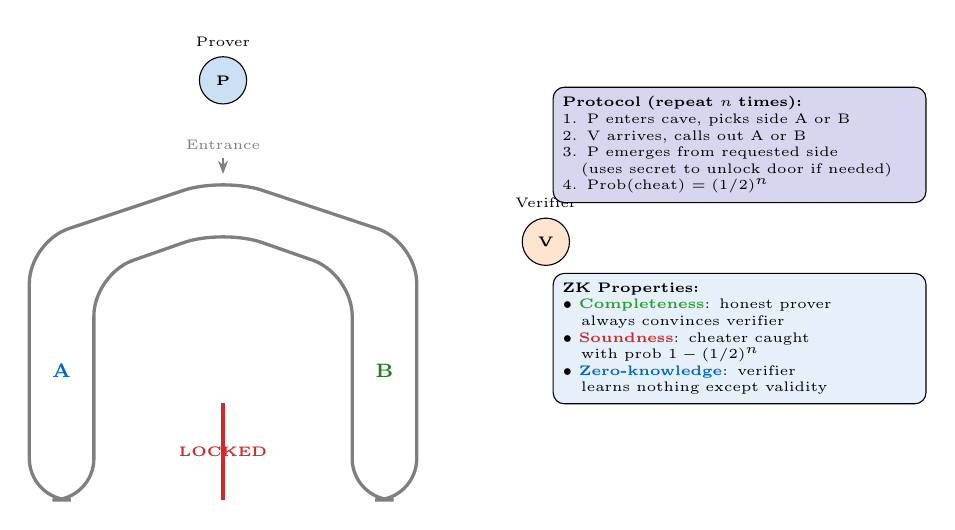
\begin{tikzpicture}[scale=0.82]
  % Cave outline
  \draw[mlgray,very thick,rounded corners=15pt] (0,0) -- (0,4) -- (3,5) -- (6,4) -- (6,0) -- (5,0) -- (5,3.5) -- (3,4.2) -- (1,3.5) -- (1,0) -- cycle;
  % Door (locked)
  \draw[mlred,very thick] (3,0) -- (3,1.5);
  \node[font=\tiny\bfseries,mlred] at (3,0.75) {LOCKED};
  % Path labels
  \node[font=\scriptsize\bfseries,mlblue] at (0.5,2) {A};
  \node[font=\scriptsize\bfseries,mlgreen!80!black] at (5.5,2) {B};
  % Entrance
  \node[font=\tiny,mlgray] at (3,5.5) {Entrance};
  \draw[-{Stealth},mlgray] (3,5.3) -- (3,5.05);
  % Prover
  \node[draw,circle,fill=mlblue!20,minimum size=0.6cm,font=\tiny\bfseries] (P) at (3,6.5) {P};
  \node[font=\tiny] at (3,7.1) {Prover};
  % Verifier
  \node[draw,circle,fill=mlorange!20,minimum size=0.6cm,font=\tiny\bfseries] (V) at (8,4) {V};
  \node[font=\tiny] at (8,4.6) {Verifier};
  % Protocol steps
  \node[draw,rounded corners,fill=mllavender4,font=\tiny,align=left,text width=4.5cm] at (11,5.5) {
    \textbf{Protocol (repeat $n$ times):}\\
    1. P enters cave, picks side A or B\\
    2. V arrives, calls out A or B\\
    3. P emerges from requested side\\
    \quad (uses secret to unlock door if needed)\\
    4. Prob(cheat) $= (1/2)^n$
  };
  % Properties
  \node[draw,rounded corners,fill=mlblue!10,font=\tiny,align=left,text width=4.5cm] at (11,2.5) {
    \textbf{ZK Properties:}\\
    $\bullet$ \textcolor{mlgreen}{\textbf{Completeness}}: honest prover\\
    \quad always convinces verifier\\
    $\bullet$ \textcolor{mlred}{\textbf{Soundness}}: cheater caught\\
    \quad with prob $1-(1/2)^n$\\
    $\bullet$ \textcolor{mlblue}{\textbf{Zero-knowledge}}: verifier\\
    \quad learns nothing except validity
  };
\end{tikzpicture}
\end{center}
\vspace{1mm}
\begin{alertblock}{Formal Definition}
\small A zero-knowledge proof for language $L$ satisfies: (1) \textbf{Completeness}: $x \in L \Rightarrow \Pr[\text{Verify accepts}] = 1$; (2) \textbf{Soundness}: $x \notin L \Rightarrow \Pr[\text{Verify accepts}] \leq \text{negl}(\lambda)$; (3) \textbf{Zero-Knowledge}: $\exists$ simulator $\mathcal{S}$ producing indistinguishable transcripts without witness.
\end{alertblock}
\bottomnote{ZK proofs: ``I can prove I know the secret without revealing the secret'' -- foundational for blockchain privacy}
\end{frame}

%--- FRAME 39: ZK-SNARKs & ZK-STARKs ---
\begin{frame}{ZK-SNARKs vs.\ ZK-STARKs}
\begin{center}
\small
\begin{tabular}{lll}
\toprule
\textbf{Property} & \textbf{ZK-SNARKs} & \textbf{ZK-STARKs} \\
\midrule
Full name & Succinct Non-interactive & Scalable Transparent \\
 & Argument of Knowledge & Argument of Knowledge \\
Trusted setup & \textcolor{mlred}{\textbf{Required}} (toxic waste) & \textcolor{mlgreen}{\textbf{Not required}} \\
Proof size & \textcolor{mlgreen}{$\sim$288 bytes (constant)} & $\sim$45--200 KB (polylog) \\
Verification time & \textcolor{mlgreen}{$\sim$10 ms (constant)} & $\sim$50--100 ms (polylog) \\
Prover time & Moderate & Moderate \\
Quantum resistance & \textcolor{mlred}{No} (relies on pairings) & \textcolor{mlgreen}{Yes} (hash-based) \\
Math basis & Elliptic curve pairings & Hash functions + FRI \\
Post-quantum & \textcolor{mlred}{Vulnerable} & \textcolor{mlgreen}{Resistant} \\
\midrule
Key deployment & Zcash, Tornado Cash, & StarkNet, StarkEx, \\
 & Filecoin, Groth16 & zkSync (hybrid) \\
\bottomrule
\end{tabular}
\end{center}
\vspace{2mm}
\begin{columns}
\column{0.48\textwidth}
\begin{block}{Trusted Setup Problem}
\begin{itemize}\small
  \item SNARKs require a ceremony generating CRS
  \item ``Toxic waste'' (secret randomness) must be destroyed
  \item If any participant is honest, setup is secure
  \item Zcash: multi-party computation ceremonies
\end{itemize}
\end{block}
\column{0.48\textwidth}
\begin{block}{Blockchain Applications}
\begin{itemize}\small
  \item \textbf{Privacy}: Zcash shielded transactions
  \item \textbf{Scaling}: zk-Rollups (Ethereum L2)
  \item \textbf{Compliance}: prove solvency without revealing balances
  \item \textbf{Identity}: prove age without revealing birthdate
\end{itemize}
\end{block}
\end{columns}
\bottomnote{Trade-off: SNARKs have smaller proofs but need trust; STARKs are transparent but proofs are larger}
\end{frame}

%--- FRAME 40: Commitment Schemes ---
\begin{frame}{Commitment Schemes}
\begin{center}
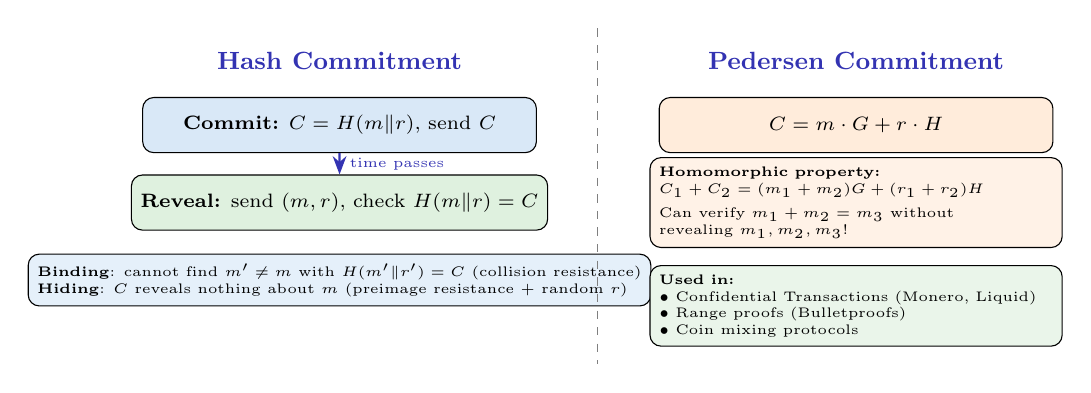
\begin{tikzpicture}[scale=0.82,
  phase/.style={draw,rounded corners,minimum width=4cm,minimum height=0.7cm,font=\scriptsize,align=center},
  arr/.style={-{Stealth},thick,mlpurple}]
  % Hash-based commitment
  \node[font=\small\bfseries,mlpurple] at (3.5,5.5) {Hash Commitment};
  % Phase 1
  \node[phase,fill=mlblue!15,minimum width=5cm] (c1) at (3.5,4.5) {\textbf{Commit:} $C = H(m \| r)$, send $C$};
  % Phase 2
  \node[phase,fill=mlgreen!15,minimum width=5cm] (c2) at (3.5,3.3) {\textbf{Reveal:} send $(m, r)$, check $H(m\|r) = C$};
  \draw[arr] (c1) -- (c2) node[midway,right,font=\tiny]{time passes};
  % Properties
  \node[draw,rounded corners,fill=mlblue!10,font=\tiny,align=left] at (3.5,2.1) {
    \textbf{Binding}: cannot find $m' \neq m$ with $H(m'\|r') = C$ (collision resistance)\\
    \textbf{Hiding}: $C$ reveals nothing about $m$ (preimage resistance + random $r$)
  };
  % Pedersen commitment
  \node[font=\small\bfseries,mlpurple] at (11.5,5.5) {Pedersen Commitment};
  \node[phase,fill=mlorange!15,minimum width=5cm] (p1) at (11.5,4.5) {$C = m \cdot G + r \cdot H$};
  \node[draw,rounded corners,fill=mlorange!10,font=\tiny,align=left,text width=5cm] at (11.5,3.3) {
    \textbf{Homomorphic property:}\\
    $C_1 + C_2 = (m_1+m_2)G + (r_1+r_2)H$\\[1mm]
    Can verify $m_1 + m_2 = m_3$ without\\
    revealing $m_1, m_2, m_3$!
  };
  \node[draw,rounded corners,fill=mlgreen!10,font=\tiny,align=left,text width=5cm] at (11.5,1.7) {
    \textbf{Used in:}\\
    $\bullet$ Confidential Transactions (Monero, Liquid)\\
    $\bullet$ Range proofs (Bulletproofs)\\
    $\bullet$ Coin mixing protocols
  };
  % Divider
  \draw[mlgray,dashed] (7.5,6) -- (7.5,0.8);
\end{tikzpicture}
\end{center}
\vspace{1mm}
\begin{alertblock}{Commitment in Blockchain}
\small Every transaction is a commitment: miners commit to a block (Merkle root) before broadcasting. Lightning HTLCs use hash commitments for atomic cross-channel payments.
\end{alertblock}
\bottomnote{Commitments are the ``sealed envelope'' of cryptography: binding and hiding until opened}
\end{frame}

%--- FRAME 41: Secret Sharing (Shamir) ---
\begin{frame}{Shamir's Secret Sharing: Mathematical Detail}
\begin{columns}
\column{0.48\textwidth}
\begin{center}
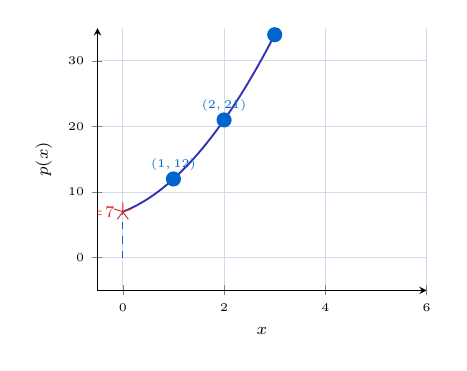
\begin{tikzpicture}[scale=0.85]
\begin{axis}[
  width=6.5cm, height=5.5cm,
  xlabel={\scriptsize $x$},
  ylabel={\scriptsize $p(x)$},
  xmin=-0.5, xmax=6,
  ymin=-5, ymax=35,
  grid=major,
  grid style={mllavender4},
  axis lines=left,
  xlabel style={font=\scriptsize},
  ylabel style={font=\scriptsize},
  tick label style={font=\tiny},
]
% Polynomial p(x) = 7 + 3x + 2x^2
\addplot[mlpurple,thick,domain=0:5.5,samples=100] {7 + 3*x + 2*x^2};
% Points (shares)
\addplot[only marks,mark=*,mlblue,mark size=3pt] coordinates {(1,12) (2,21) (3,34)};
\addplot[only marks,mark=*,mlgreen,mark size=3pt] coordinates {(4,51)};
\addplot[only marks,mark=*,mlorange,mark size=3pt] coordinates {(5,72)};
% Labels
\node[font=\tiny,mlblue,above] at (axis cs:1,12) {$(1,12)$};
\node[font=\tiny,mlblue,above] at (axis cs:2,21) {$(2,21)$};
\node[font=\tiny,mlblue,above left] at (axis cs:3,34) {$(3,34)$};
\node[font=\tiny,mlgreen,below right] at (axis cs:4,51) {$(4,51)$};
\node[font=\tiny,mlorange,below right] at (axis cs:5,72) {$(5,72)$};
% Secret
\addplot[only marks,mark=star,mlred,mark size=4pt] coordinates {(0,7)};
\node[font=\scriptsize\bfseries,mlred,left] at (axis cs:0,7) {$S\!=\!7$};
% Annotation
\draw[mlblue,dashed] (axis cs:0,0) -- (axis cs:0,7);
\end{axis}
\end{tikzpicture}
\end{center}
\column{0.48\textwidth}
\begin{block}{Construction ($t$-of-$n$)}
\small
\begin{enumerate}\scriptsize
  \item Secret $S = p(0)$, pick random $a_1, \ldots, a_{t-1}$
  \item Polynomial: $p(x) = S + a_1 x + \cdots + a_{t-1} x^{t-1}$
  \item Share $i$: $(i, p(i))$ for $i = 1, \ldots, n$
  \item Any $t$ shares $\to$ Lagrange interpolation $\to$ $p(0) = S$
\end{enumerate}
\end{block}
\vspace{1mm}
\begin{block}{Lagrange Interpolation}
\small Given points $(x_1,y_1), \ldots, (x_t,y_t)$:
\[
  S = p(0) = \sum_{i=1}^{t} y_i \prod_{\substack{j=1\\j\neq i}}^{t} \frac{-x_j}{x_i - x_j}
\]
All arithmetic in $\mathbb{F}_p$ (finite field).
\end{block}
\vspace{1mm}
\begin{alertblock}{Security}
\small $t\!-\!1$ shares give \emph{no information}: any secret is equally consistent with $t\!-\!1$ points (infinite polynomials pass through $t\!-\!1$ points).
\end{alertblock}
\end{columns}
\bottomnote{Example: $p(x) = 7 + 3x + 2x^2$ (secret $= 7$, threshold $= 3$); any 3 of 5 shares recover the secret}
\end{frame}

%--- FRAME 42: Homomorphic Encryption Basics ---
\begin{frame}{Homomorphic Encryption Basics}
\begin{block}{Definition}
\small A homomorphic encryption scheme allows computation on ciphertexts: $\text{Dec}(f(\text{Enc}(m_1), \text{Enc}(m_2))) = f(m_1, m_2)$ without decrypting.
\end{block}
\vspace{2mm}
\begin{columns}
\column{0.48\textwidth}
\begin{block}{Types of Homomorphic Encryption}
\small
\begin{tabular}{lll}
\toprule
\textbf{Type} & \textbf{Operations} & \textbf{Example} \\
\midrule
Partial (PHE) & One type & RSA ($\times$) \\
 & & Paillier ($+$) \\
 & & ElGamal ($\times$) \\
\midrule
Somewhat & Both, limited & BGN \\
(SHE) & depth & \\
\midrule
Fully (FHE) & Both, & TFHE, \\
 & unlimited & CKKS \\
\bottomrule
\end{tabular}
\end{block}
\column{0.48\textwidth}
\begin{block}{Practical Considerations}
\begin{itemize}\small
  \item FHE: $\sim 10{,}000\!\times$ slower than plaintext operations
  \item Ciphertext expansion: $\sim 100\!\times$ size increase
  \item Bootstrapping: refresh noise for unlimited depth
  \item Active research: TFHE, CKKS improving rapidly
\end{itemize}
\end{block}
\vspace{1mm}
\begin{block}{Blockchain Applications}
\begin{itemize}\small
  \item \textbf{Private smart contracts}: compute on encrypted state
  \item \textbf{Encrypted auctions}: bid without revealing price
  \item \textbf{Private voting}: tally without decrypting votes
  \item Fhenix, Zama: FHE-enabled blockchains
\end{itemize}
\end{block}
\end{columns}
\vspace{1mm}
\begin{alertblock}{RSA Multiplicative Homomorphism}
\small $\text{Enc}(m_1) \cdot \text{Enc}(m_2) = m_1^e \cdot m_2^e = (m_1 m_2)^e = \text{Enc}(m_1 \cdot m_2) \pmod{n}$
\end{alertblock}
\bottomnote{FHE is the ``holy grail'' of encryption -- practical FHE would enable fully private computation on public blockchains}
\end{frame}

%--- FRAME 43: Ring Signatures & Stealth Addresses ---
\begin{frame}{Ring Signatures \& Stealth Addresses}
\begin{center}
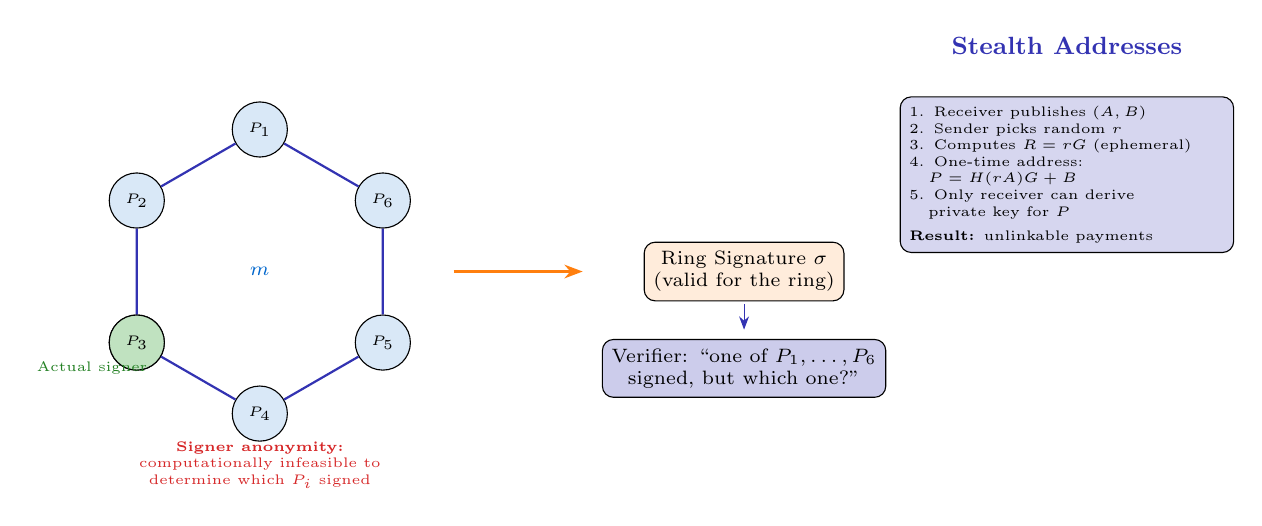
\begin{tikzpicture}[scale=0.82,
  key/.style={draw,circle,fill=mlblue!15,minimum size=0.7cm,font=\tiny}]
  % Ring of public keys
  \def\n{6}
  \def\radius{2.2}
  \foreach \i in {1,...,\n}{
    \pgfmathsetmacro{\angle}{90 + (\i-1)*360/\n}
    \node[key] (k\i) at (\angle:\radius) {$P_{\i}$};
  }
  % Highlight actual signer
  \node[draw,circle,fill=mlgreen!30,minimum size=0.7cm,font=\tiny\bfseries] at (90+2*360/6:2.2) {$P_{3}$};
  \node[font=\tiny,mlgreen!80!black] at (90+2*360/6:3) {Actual signer};
  % Ring connections
  \foreach \i in {1,...,\n}{
    \pgfmathtruncatemacro{\j}{mod(\i,\n)+1}
    \draw[mlpurple,thick] (k\i) -- (k\j);
  }
  % Message input
  \node[font=\scriptsize,mlblue] at (0,0) {$m$};
  % Output
  \draw[-{Stealth},thick,mlorange] (3,0) -- (5,0);
  \node[draw,rounded corners,fill=mlorange!15,font=\scriptsize,align=center] at (7.5,0) {Ring Signature $\sigma$\\(valid for the ring)};
  % Verifier
  \node[draw,rounded corners,fill=mllavender3,font=\scriptsize,align=center] at (7.5,-1.5) {Verifier: ``one of $P_1,\ldots,P_6$\\signed, but which one?''};
  \draw[-{Stealth},mlpurple] (7.5,-0.5) -- (7.5,-0.9);
  % Key property
  \node[font=\tiny,mlred,align=center] at (0,-3) {\textbf{Signer anonymity:}\\computationally infeasible to\\determine which $P_i$ signed};
  % Stealth addresses (right side)
  \node[font=\small\bfseries,mlpurple] at (12.5,3.5) {Stealth Addresses};
  \node[draw,rounded corners,fill=mllavender4,font=\tiny,align=left,text width=4cm] at (12.5,1.5) {
    1. Receiver publishes $(A,B)$\\
    2. Sender picks random $r$\\
    3. Computes $R = rG$ (ephemeral)\\
    4. One-time address:\\
    \quad $P = H(rA)G + B$\\
    5. Only receiver can derive\\
    \quad private key for $P$\\[1mm]
    \textbf{Result:} unlinkable payments
  };
\end{tikzpicture}
\end{center}
\vspace{1mm}
\begin{columns}
\column{0.48\textwidth}
\begin{block}{Monero Privacy Stack}
\begin{itemize}\small
  \item \textbf{Ring signatures}: hide sender among decoys
  \item \textbf{Stealth addresses}: one-time recipient addresses
  \item \textbf{RingCT}: confidential transaction amounts
  \item Combined: sender, receiver, and amount all hidden
\end{itemize}
\end{block}
\column{0.48\textwidth}
\begin{block}{Trade-offs}
\begin{itemize}\small
  \item Ring size $\uparrow$ $\to$ privacy $\uparrow$, tx size $\uparrow$
  \item Monero ring size: 16 (mandatory)
  \item Larger transactions $=$ higher fees
  \item Regulatory tension: privacy vs.\ compliance
\end{itemize}
\end{block}
\end{columns}
\bottomnote{Ring signatures (Rivest--Shamir--Tauman, 2001): signer-ambiguous signatures -- the basis of Monero's privacy}
\end{frame}

\section{Attacks \& Post-Quantum Cryptography}

%--- FRAME 44: Birthday Attack Detailed ---
\begin{frame}{Birthday Attack: Complexity Analysis}
\begin{center}
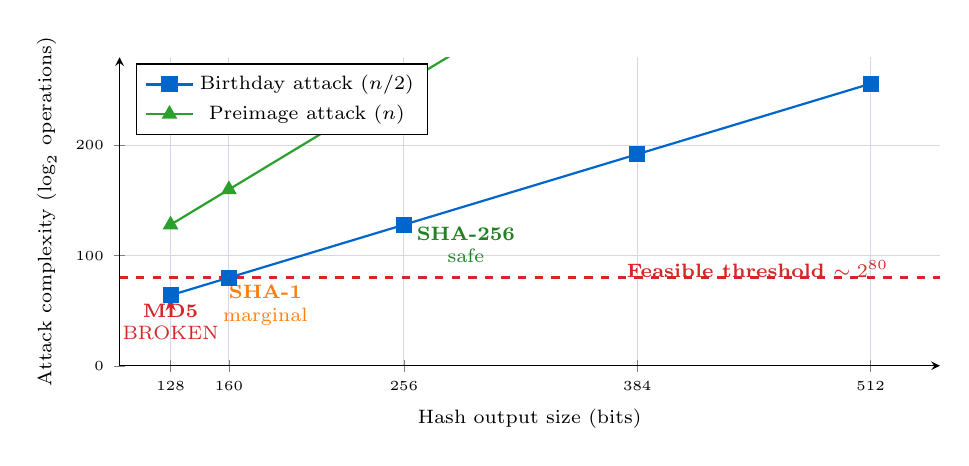
\begin{tikzpicture}
\begin{axis}[
  width=12cm, height=5.5cm,
  xlabel={\scriptsize Hash output size (bits)},
  ylabel={\scriptsize Attack complexity ($\log_2$ operations)},
  xmin=100, xmax=550,
  ymin=0, ymax=280,
  grid=major,
  grid style={mllavender4},
  axis lines=left,
  xlabel style={font=\scriptsize},
  ylabel style={font=\scriptsize},
  tick label style={font=\tiny},
  legend style={font=\scriptsize,at={(0.02,0.98)},anchor=north west},
  xtick={128,160,256,384,512},
]
% Birthday attack: n/2
\addplot[mlblue,thick,mark=square*,mark size=2.5pt] coordinates {
  (128,64) (160,80) (256,128) (384,192) (512,256)
};
\addlegendentry{Birthday attack ($n/2$)}
% Preimage attack: n
\addplot[mlgreen,thick,mark=triangle*,mark size=2.5pt] coordinates {
  (128,128) (160,160) (256,256) (384,384) (512,512)
};
\addlegendentry{Preimage attack ($n$)}
% Feasible threshold
\draw[mlred,dashed,very thick] (axis cs:100,80) -- (axis cs:550,80);
\node[font=\scriptsize\bfseries,mlred] at (axis cs:450,88) {Feasible threshold $\sim 2^{80}$};
% MD5 label
\node[font=\scriptsize,mlred,align=center] at (axis cs:128,40) {\textbf{MD5}\\BROKEN};
\draw[-{Stealth},mlred] (axis cs:128,50) -- (axis cs:128,62);
% SHA-1 label
\node[font=\scriptsize,mlorange,align=center] at (axis cs:180,55) {\textbf{SHA-1}\\marginal};
% SHA-256 label
\node[font=\scriptsize,mlgreen!80!black,align=center] at (axis cs:290,110) {\textbf{SHA-256}\\safe};
\end{axis}
\end{tikzpicture}
\end{center}
\vspace{1mm}
\begin{columns}
\column{0.48\textwidth}
\begin{block}{Attack History}
\begin{itemize}\small
  \item \textbf{MD5} (128-bit): collision in $2^{24}$ -- seconds on laptop
  \item \textbf{SHA-1} (160-bit): SHAttered attack (2017, $2^{63}$)
  \item \textbf{SHA-256} (256-bit): $2^{128}$ -- safe for decades
\end{itemize}
\end{block}
\column{0.48\textwidth}
\begin{block}{Implications for Blockchain}
\begin{itemize}\small
  \item Bitcoin addresses use RIPEMD-160: birthday at $2^{80}$
  \item But address collision requires matching private key
  \item SHA-256 for block hashing: $2^{128}$ birthday bound
  \item Grover's algorithm: halves exponent (post-quantum)
\end{itemize}
\end{block}
\end{columns}
\bottomnote{Rule of thumb: hash output must be $\geq 2\times$ desired security level due to the birthday bound}
\end{frame}

%--- FRAME 45: Length Extension Attack ---
\begin{frame}{Length Extension Attack \& HMAC Defense}
\begin{center}
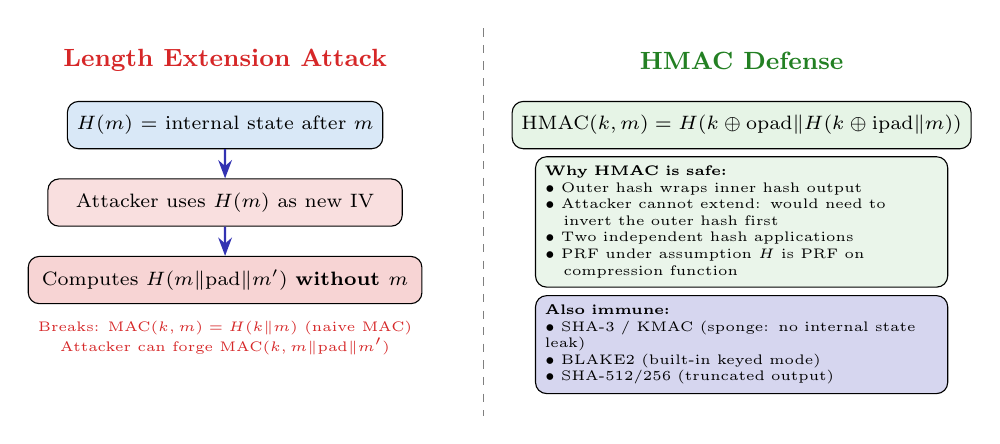
\begin{tikzpicture}[scale=0.82,
  box/.style={draw,rounded corners,minimum width=3cm,minimum height=0.6cm,font=\scriptsize,align=center},
  arr/.style={-{Stealth},thick,mlpurple}]
  % Attack diagram
  \node[font=\small\bfseries,mlred] at (4,5.5) {Length Extension Attack};
  \node[box,fill=mlblue!15] (h1) at (4,4.5) {$H(m)$ = internal state after $m$};
  \node[box,fill=mlred!15,minimum width=4.5cm] (ext) at (4,3.3) {Attacker uses $H(m)$ as new IV};
  \draw[arr] (h1) -- (ext);
  \node[box,fill=mlred!20,minimum width=5cm] (forge) at (4,2.1) {Computes $H(m \| \text{pad} \| m')$ \textbf{without $m$}};
  \draw[arr] (ext) -- (forge);
  \node[font=\tiny,mlred,align=center] at (4,1.2) {Breaks: $\text{MAC}(k,m) = H(k \| m)$ (naive MAC)\\Attacker can forge $\text{MAC}(k, m \| \text{pad} \| m')$};
  % HMAC defense
  \node[font=\small\bfseries,mlgreen!80!black] at (12,5.5) {HMAC Defense};
  \node[box,fill=mlgreen!12,minimum width=5cm] (hmac) at (12,4.5) {$\text{HMAC}(k,m) = H(k \oplus \text{opad} \| H(k \oplus \text{ipad} \| m))$};
  \node[draw,rounded corners,fill=mlgreen!10,font=\tiny,align=left,text width=5cm] at (12,3) {
    \textbf{Why HMAC is safe:}\\
    $\bullet$ Outer hash wraps inner hash output\\
    $\bullet$ Attacker cannot extend: would need to\\
    \quad invert the outer hash first\\
    $\bullet$ Two independent hash applications\\
    $\bullet$ PRF under assumption $H$ is PRF on\\
    \quad compression function
  };
  \node[draw,rounded corners,fill=mllavender4,font=\tiny,align=left,text width=5cm] at (12,1.1) {
    \textbf{Also immune:}\\
    $\bullet$ SHA-3 / KMAC (sponge: no internal state leak)\\
    $\bullet$ BLAKE2 (built-in keyed mode)\\
    $\bullet$ SHA-512/256 (truncated output)
  };
  % Divider
  \draw[mlgray,dashed] (8,6) -- (8,0);
\end{tikzpicture}
\end{center}
\vspace{1mm}
\begin{alertblock}{Practical Impact}
\small Flickr API (2009) used $H(\text{secret} \| \text{params})$ -- vulnerable to forgery. Any Merkle--Damg\r{a}rd hash with $H(k\|m)$ as MAC is broken. Always use HMAC or a keyed hash mode.
\end{alertblock}
\bottomnote{Length extension exploits Merkle--Damg\r{a}rd's iterative structure -- the internal state after hashing IS the hash output}
\end{frame}

%--- FRAME 46: Side-Channel Attacks ---
\begin{frame}{Side-Channel Attacks on Cryptographic Implementations}
\begin{center}
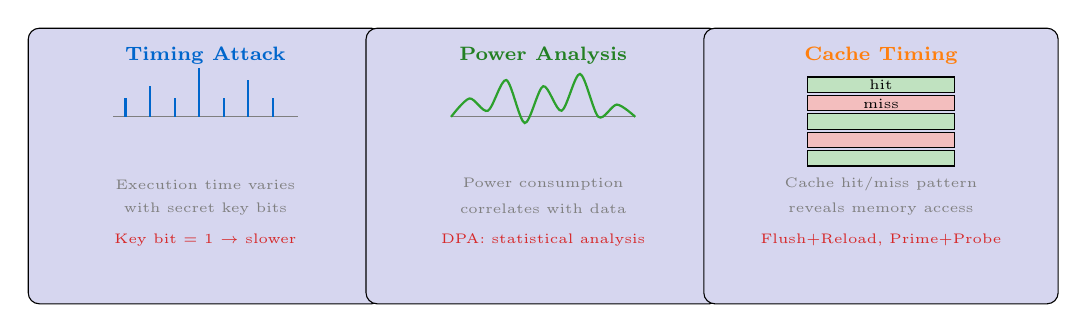
\begin{tikzpicture}[scale=0.78,
  panel/.style={draw,rounded corners,fill=mllavender4,minimum width=4.5cm,minimum height=3.5cm,align=center}]
  % Panel 1: Timing
  \node[panel] (p1) at (0,0) {};
  \node[font=\scriptsize\bfseries,mlblue] at (0,1.8) {Timing Attack};
  % Simulated timing trace
  \draw[mlgray,thin] (-1.5,0.8) -- (1.5,0.8);
  \foreach \x/\h in {-1.3/0.3,-0.9/0.5,-0.5/0.3,-0.1/0.8,0.3/0.3,0.7/0.6,1.1/0.3}{
    \draw[mlblue,thick] (\x,0.8) -- (\x,{0.8+\h});
  }
  \node[font=\tiny,mlgray] at (0,-0.3) {Execution time varies};
  \node[font=\tiny,mlgray] at (0,-0.7) {with secret key bits};
  \node[font=\tiny,mlred] at (0,-1.2) {Key bit = 1 $\to$ slower};
  % Panel 2: Power
  \node[panel] (p2) at (5.5,0) {};
  \node[font=\scriptsize\bfseries,mlgreen!80!black] at (5.5,1.8) {Power Analysis};
  % Simulated power trace
  \draw[mlgray,thin] (4,0.8) -- (7,0.8);
  \draw[mlgreen,thick] plot[smooth] coordinates {(4,0.8)(4.3,1.1)(4.6,0.9)(4.9,1.4)(5.2,0.7)(5.5,1.3)(5.8,0.9)(6.1,1.5)(6.4,0.8)(6.7,1.0)(7,0.8)};
  \node[font=\tiny,mlgray] at (5.5,-0.3) {Power consumption};
  \node[font=\tiny,mlgray] at (5.5,-0.7) {correlates with data};
  \node[font=\tiny,mlred] at (5.5,-1.2) {DPA: statistical analysis};
  % Panel 3: Cache
  \node[panel] (p3) at (11,0) {};
  \node[font=\scriptsize\bfseries,mlorange] at (11,1.8) {Cache Timing};
  % Cache pattern
  \foreach \y/\c in {1.2/mlgreen!30,0.9/mlred!30,0.6/mlgreen!30,0.3/mlred!30,0.0/mlgreen!30}{
    \draw[fill=\c] (9.8,\y) rectangle (12.2,{\y+0.25});
  }
  \node[font=\tiny] at (11,1.32) {\tiny hit};
  \node[font=\tiny] at (11,1.02) {\tiny miss};
  \node[font=\tiny,mlgray] at (11,-0.3) {Cache hit/miss pattern};
  \node[font=\tiny,mlgray] at (11,-0.7) {reveals memory access};
  \node[font=\tiny,mlred] at (11,-1.2) {Flush+Reload, Prime+Probe};
\end{tikzpicture}
\end{center}
\vspace{2mm}
\begin{columns}
\column{0.48\textwidth}
\begin{block}{Mitigations}
\begin{itemize}\small
  \item \textbf{Constant-time code}: no secret-dependent branches
  \item \textbf{Masking}: randomize intermediate values
  \item \textbf{Shielding}: Faraday cages, power filtering
  \item \textbf{Blinding}: randomize inputs before computation
\end{itemize}
\end{block}
\column{0.48\textwidth}
\begin{block}{Notable Attacks}
\begin{itemize}\small
  \item \textbf{Spectre/Meltdown}: CPU speculation leaks
  \item \textbf{ECDSA timing}: OpenSSL key extraction (2011)
  \item \textbf{AES cache}: full key recovery in minutes
  \item \textbf{Power analysis}: smartcard key extraction
\end{itemize}
\end{block}
\end{columns}
\bottomnote{Side-channels attack the \emph{implementation}, not the \emph{algorithm} -- correct code with wrong timing is still broken}
\end{frame}

%--- FRAME 47: Quantum Computing: Shor's Algorithm ---
\begin{frame}{Quantum Threat: Shor's Algorithm}
\begin{center}
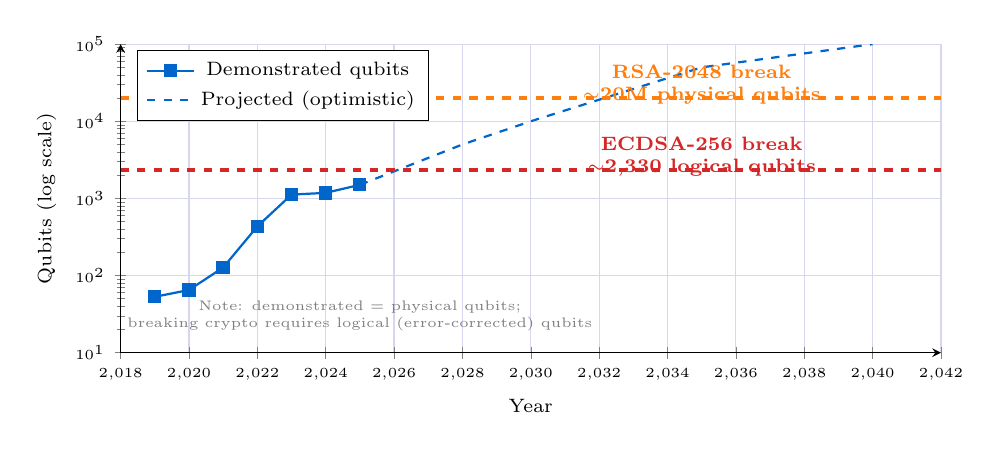
\begin{tikzpicture}
\begin{axis}[
  width=12cm, height=5.5cm,
  xlabel={\scriptsize Year},
  ylabel={\scriptsize Qubits (log scale)},
  xmin=2018, xmax=2042,
  ymin=10, ymax=100000,
  ymode=log,
  grid=major,
  grid style={mllavender4},
  axis lines=left,
  xlabel style={font=\scriptsize},
  ylabel style={font=\scriptsize},
  tick label style={font=\tiny},
  legend style={font=\scriptsize,at={(0.02,0.98)},anchor=north west},
]
% Actual progress + projection
\addplot[mlblue,thick,mark=square*,mark size=2pt] coordinates {
  (2019,53) (2020,65) (2021,127) (2022,433) (2023,1121) (2024,1180) (2025,1500)
};
\addlegendentry{Demonstrated qubits}
% Projected growth
\addplot[mlblue,thick,dashed,mark=none] coordinates {
  (2025,1500) (2028,5000) (2030,10000) (2035,50000) (2040,100000)
};
\addlegendentry{Projected (optimistic)}
% ECDSA-256 break threshold
\draw[mlred,very thick,dashed] (axis cs:2018,2330) -- (axis cs:2042,2330);
\node[font=\scriptsize\bfseries,mlred,align=center] at (axis cs:2035,3500) {ECDSA-256 break\\$\sim$2{,}330 logical qubits};
% RSA-2048 break threshold
\draw[mlorange,very thick,dashed] (axis cs:2018,20000) -- (axis cs:2042,20000);
\node[font=\scriptsize\bfseries,mlorange,align=center] at (axis cs:2035,30000) {RSA-2048 break\\$\sim$20M physical qubits};
% Note
\node[font=\tiny,mlgray,align=center] at (axis cs:2025,30) {Note: demonstrated = physical qubits;\\breaking crypto requires logical (error-corrected) qubits};
\end{axis}
\end{tikzpicture}
\end{center}
\vspace{1mm}
\begin{columns}
\column{0.48\textwidth}
\begin{block}{What Shor's Algorithm Breaks}
\begin{itemize}\small
  \item \textbf{RSA}: factors $n=pq$ in $\mathcal{O}((\log n)^3)$
  \item \textbf{ECDSA/EdDSA}: solves ECDLP in $\mathcal{O}((\log n)^3)$
  \item \textbf{DH/ECDH}: computes discrete log
  \item All current public-key crypto is vulnerable
\end{itemize}
\end{block}
\column{0.48\textwidth}
\begin{block}{Timeline Estimates}
\begin{itemize}\small
  \item \textbf{2025}: $\sim$1{,}500 noisy physical qubits
  \item \textbf{2030--2035}: possible cryptographically relevant QC
  \item \textbf{Harvest now, decrypt later}: adversaries storing data today
  \item Migration should begin \textbf{now}
\end{itemize}
\end{block}
\end{columns}
\bottomnote{Shor (1994): polynomial-time quantum algorithm for factoring and discrete log -- existential threat to current PKI}
\end{frame}

%--- FRAME 48: Quantum Computing: Grover's Algorithm ---
\begin{frame}{Grover's Algorithm: Impact on Symmetric Crypto}
\begin{block}{Grover's Algorithm}
\small Quantum search over $N$ elements in $\mathcal{O}(\sqrt{N})$ time vs.\ $\mathcal{O}(N)$ classically. Effectively halves the security parameter of symmetric primitives.
\end{block}
\vspace{3mm}
\begin{center}
\small
\begin{tabular}{llll}
\toprule
\textbf{Algorithm} & \textbf{Classical Security} & \textbf{Post-Quantum Security} & \textbf{Recommendation} \\
\midrule
AES-128 & $2^{128}$ & $2^{64}$ (\textcolor{mlred}{insufficient}) & Upgrade to AES-256 \\
AES-192 & $2^{192}$ & $2^{96}$ (marginal) & Acceptable for now \\
AES-256 & $2^{256}$ & $2^{128}$ (\textcolor{mlgreen}{safe}) & \textcolor{mlgreen}{\textbf{Recommended}} \\
SHA-256 (preimage) & $2^{256}$ & $2^{128}$ (\textcolor{mlgreen}{safe}) & No change needed \\
SHA-256 (collision) & $2^{128}$ & $2^{85}$ (marginal) & Consider SHA-384+ \\
HMAC-SHA-256 & $2^{128}$ & $2^{85}$ (marginal) & Consider HMAC-SHA-512 \\
ChaCha20 (256-bit) & $2^{256}$ & $2^{128}$ (\textcolor{mlgreen}{safe}) & \textcolor{mlgreen}{\textbf{Recommended}} \\
\bottomrule
\end{tabular}
\end{center}
\vspace{3mm}
\begin{columns}
\column{0.48\textwidth}
\begin{block}{Key Insight}
\begin{itemize}\small
  \item Grover is a \textbf{square-root speedup} only
  \item Unlike Shor, does not break symmetric crypto
  \item Solution: double the key size
\end{itemize}
\end{block}
\column{0.48\textwidth}
\begin{block}{Bitcoin Impact}
\begin{itemize}\small
  \item SHA-256 mining: $2^{128}$ post-quantum -- safe
  \item RIPEMD-160 addresses: $2^{80}$ preimage -- marginal
  \item ECDSA: broken by Shor (not Grover)
  \item Priority: replace signatures, not hashes
\end{itemize}
\end{block}
\end{columns}
\bottomnote{Grover (1996): generic quantum speedup -- symmetric crypto survives by doubling key sizes}
\end{frame}

%--- FRAME 49: Post-Quantum Cryptography Candidates ---
\begin{frame}{Post-Quantum Cryptography: NIST Standards}
\begin{center}
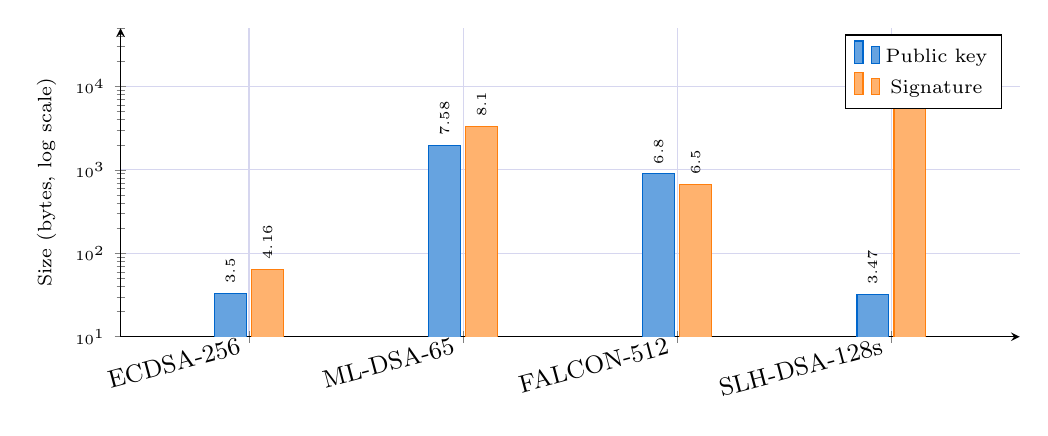
\begin{tikzpicture}
\begin{axis}[
  ybar,
  width=13cm, height=5.5cm,
  ylabel={\scriptsize Size (bytes, log scale)},
  ymode=log,
  symbolic x coords={ECDSA-256,ML-DSA-65,FALCON-512,SLH-DSA-128s},
  xtick=data,
  x tick label style={font=\small,rotate=15,anchor=east},
  y tick label style={font=\tiny},
  ymin=10, ymax=50000,
  bar width=0.4cm,
  axis lines=left,
  grid=major,
  grid style={mllavender4},
  ylabel style={font=\scriptsize},
  legend style={font=\scriptsize,at={(0.98,0.98)},anchor=north east},
  nodes near coords,
  nodes near coords style={font=\tiny,rotate=90,anchor=west},
  enlarge x limits=0.2,
]
\addplot[fill=mlblue!60,draw=mlblue] coordinates {
  (ECDSA-256,33) (ML-DSA-65,1952) (FALCON-512,897) (SLH-DSA-128s,32)
};
\addlegendentry{Public key}
\addplot[fill=mlorange!60,draw=mlorange] coordinates {
  (ECDSA-256,64) (ML-DSA-65,3293) (FALCON-512,666) (SLH-DSA-128s,7856)
};
\addlegendentry{Signature}
\end{axis}
\end{tikzpicture}
\end{center}
\vspace{1mm}
\begin{columns}
\column{0.48\textwidth}
\begin{block}{NIST PQC Standards (2024)}
\scriptsize
\begin{tabular}{lll}
\toprule
\textbf{Standard} & \textbf{Basis} & \textbf{Type} \\
\midrule
ML-KEM & Lattices (MLWE) & Key encapsulation \\
ML-DSA & Lattices (MLWE) & Digital signature \\
SLH-DSA & Hash-based & Digital signature \\
FN-DSA & Lattices (NTRU) & Digital signature \\
\bottomrule
\end{tabular}
\end{block}
\column{0.48\textwidth}
\begin{block}{Blockchain Challenges}
\begin{itemize}\small
  \item \textbf{Size}: PQ signatures are $10$--$100\times$ larger
  \item \textbf{On-chain cost}: every byte is permanent and replicated
  \item \textbf{Compatibility}: address format changes needed
  \item \textbf{Performance}: lattice ops are fast; hash-based are slower
\end{itemize}
\end{block}
\end{columns}
\bottomnote{NIST finalized ML-DSA (Dilithium), ML-KEM (Kyber), and SLH-DSA (SPHINCS+) as first post-quantum standards in 2024}
\end{frame}

%--- FRAME 50: Blockchain Post-Quantum Migration ---
\begin{frame}{Blockchain Post-Quantum Migration Roadmap}
\begin{center}
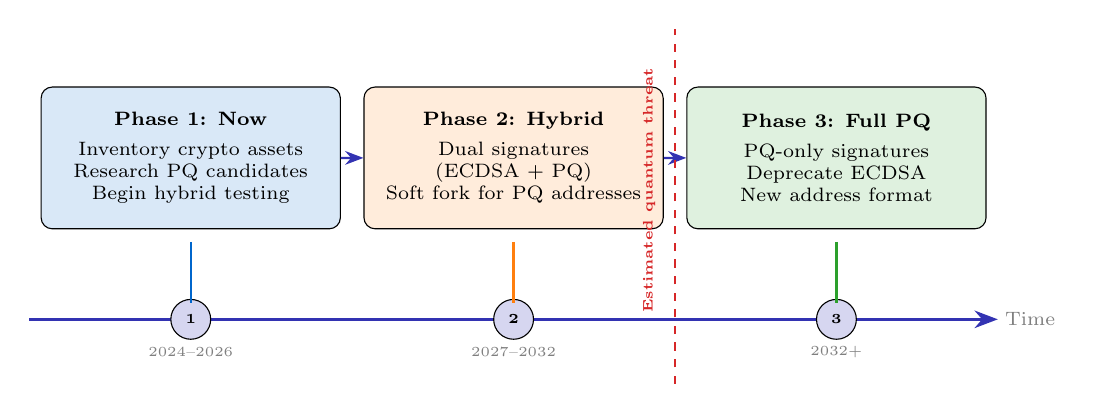
\begin{tikzpicture}[scale=0.82,
  phasebox/.style={draw,rounded corners,minimum width=3.8cm,minimum height=1.8cm,font=\scriptsize,align=center},
  milestone/.style={draw,circle,fill=mlpurple!20,minimum size=0.5cm,font=\tiny\bfseries}]
  % Timeline arrow
  \draw[-{Stealth},very thick,mlpurple] (0,0) -- (15,0);
  \node[font=\scriptsize,mlgray] at (15.5,0) {Time};
  % Phase 1: Current
  \node[phasebox,fill=mlblue!15] (p1) at (2.5,2.5) {\textbf{Phase 1: Now}\\[1mm]Inventory crypto assets\\Research PQ candidates\\Begin hybrid testing};
  \node[milestone] at (2.5,0) {1};
  \node[font=\tiny,mlgray] at (2.5,-0.5) {2024--2026};
  \draw[mlblue,thick] (2.5,1.2) -- (2.5,0.25);
  % Phase 2: Hybrid
  \node[phasebox,fill=mlorange!15] (p2) at (7.5,2.5) {\textbf{Phase 2: Hybrid}\\[1mm]Dual signatures\\(ECDSA + PQ)\\Soft fork for PQ addresses};
  \node[milestone] at (7.5,0) {2};
  \node[font=\tiny,mlgray] at (7.5,-0.5) {2027--2032};
  \draw[mlorange,thick] (7.5,1.2) -- (7.5,0.25);
  % Phase 3: Full PQ
  \node[phasebox,fill=mlgreen!15] (p3) at (12.5,2.5) {\textbf{Phase 3: Full PQ}\\[1mm]PQ-only signatures\\Deprecate ECDSA\\New address format};
  \node[milestone] at (12.5,0) {3};
  \node[font=\tiny,mlgray] at (12.5,-0.5) {2032+};
  \draw[mlgreen,thick] (12.5,1.2) -- (12.5,0.25);
  % Arrows between phases
  \draw[-{Stealth},thick,mlpurple] (p1) -- (p2);
  \draw[-{Stealth},thick,mlpurple] (p2) -- (p3);
  % Threat line
  \draw[mlred,thick,dashed] (10,-1) -- (10,4.5);
  \node[font=\tiny\bfseries,mlred,rotate=90] at (9.6,2) {Estimated quantum threat};
\end{tikzpicture}
\end{center}
\vspace{2mm}
\begin{columns}
\column{0.48\textwidth}
\begin{block}{Migration Challenges}
\begin{itemize}\small
  \item \textbf{Consensus}: hard/soft fork for new sig types
  \item \textbf{Lost coins}: addresses with lost keys cannot migrate
  \item \textbf{Backward compatibility}: support old and new formats
  \item \textbf{Testing}: PQ schemes less battle-tested
\end{itemize}
\end{block}
\column{0.48\textwidth}
\begin{block}{Current Initiatives}
\begin{itemize}\small
  \item \textbf{Bitcoin}: BIP proposals for PQ addresses (research)
  \item \textbf{Ethereum}: EIP-7693 (PQ account abstraction)
  \item \textbf{QRL}: quantum-resistant ledger (XMSS signatures)
  \item \textbf{NIST}: PQ standards finalized (Aug 2024)
\end{itemize}
\end{block}
\end{columns}
\bottomnote{``Harvest now, decrypt later'' -- the migration to post-quantum cryptography is urgent even before quantum computers arrive}
\end{frame}

%--- FRAME 51: Summary & Key Formulas ---
\begin{frame}{Summary \& Key Formulas}
\begin{columns}
\column{0.48\textwidth}
\begin{block}{Hash Functions}
\scriptsize
\begin{itemize}
  \item Preimage: $\mathcal{O}(2^n)$ \quad Collision: $\mathcal{O}(2^{n/2})$
  \item SHA-256: 64 rounds, 512-bit blocks, 256-bit digest
  \item Sponge (SHA-3): $b = r + c$, no length extension
\end{itemize}
\end{block}
\vspace{1mm}
\begin{block}{ECDSA (secp256k1)}
\scriptsize
\begin{itemize}
  \item Key: $d \in [1,n\!-\!1]$, $Q = dG$
  \item Sign: $r = (kG)_x$, $s = k^{-1}(e + dr)$
  \item Verify: $u_1 G + u_2 Q$, check $x = r$
  \item Security: $2^{128}$ (Pollard's rho)
\end{itemize}
\end{block}
\vspace{1mm}
\begin{block}{Schnorr}
\scriptsize
\begin{itemize}
  \item Sign: $R = kG$, $e = H(R\|P\|m)$, $s = k - ed$
  \item Verify: $sG = R - eP$
  \item Key advantage: linearity $\to$ aggregation
\end{itemize}
\end{block}
\column{0.48\textwidth}
\begin{block}{Diffie--Hellman}
\scriptsize
\begin{itemize}
  \item Shared secret: $s = g^{ab} \bmod p$
  \item DDH assumption: $(g^a, g^b, g^{ab})$ vs.\ $(g^a, g^b, g^c)$
\end{itemize}
\end{block}
\vspace{1mm}
\begin{block}{Shamir's Secret Sharing}
\scriptsize
\begin{itemize}
  \item $p(x) = S + a_1 x + \cdots + a_{t-1}x^{t-1}$
  \item $t$ points $\to$ Lagrange interpolation $\to$ $S = p(0)$
  \item $t\!-\!1$ shares: zero information
\end{itemize}
\end{block}
\vspace{1mm}
\begin{block}{Post-Quantum}
\scriptsize
\begin{itemize}
  \item Shor: breaks RSA, ECDSA in $\mathcal{O}((\log n)^3)$
  \item Grover: $\sqrt{N}$ search $\to$ double symmetric key sizes
  \item NIST PQC: ML-DSA (lattice), SLH-DSA (hash)
\end{itemize}
\end{block}
\vspace{1mm}
\begin{block}{Key Takeaways}
\scriptsize
\begin{enumerate}
  \item ECC: compact keys, fast ops, proven security
  \item Nonce reuse = total key compromise
  \item HD wallets: one seed, unlimited keys
  \item Post-quantum migration: start planning now
\end{enumerate}
\end{block}
\end{columns}
\bottomnote{These formulas and bounds form the quantitative foundation of blockchain cryptographic security}
\end{frame}

%--- FRAME 52: Questions & Discussion ---
\begin{frame}{Questions \& Discussion}
\begin{block}{Open Questions for Discussion}
\begin{enumerate}\large
  \item \textbf{When will quantum computers threaten Bitcoin?}\\[2mm]
    \small Given current qubit progress ($\sim$1{,}500 in 2025) and the $\sim$2{,}330 logical qubits needed for ECDSA-256, what is a realistic timeline? How should the Bitcoin community prepare?
  \vspace{3mm}
  \item \textbf{Is perfect privacy possible on a public blockchain?}\\[2mm]
    \small Ring signatures, zk-SNARKs, and stealth addresses provide strong privacy. Can we achieve both full transparency (for auditing) and full privacy (for users) simultaneously?
  \vspace{3mm}
  \item \textbf{Usability vs.\ security in key management?}\\[2mm]
    \small 24-word seed phrases, hardware wallets, and Shamir splits maximize security but create friction. How do we make self-custody accessible to non-technical users without compromising security?
\end{enumerate}
\end{block}
\vspace{4mm}
\begin{center}
\textcolor{mlpurple}{\Large\textbf{Thank you!}}\\[2mm]
\textcolor{mlgray}{\small Prof.~Dr.~Joerg Osterrieder}
\end{center}
\end{frame}

\end{document}
